\documentclass[12pt]{book}
\usepackage{booktabs}
\usepackage[table]{xcolor}
\usepackage{tcolorbox}
\usepackage[T1]{fontenc}
\usepackage{wrapfig}
\usepackage{url}
\usepackage{dsfont}
\usepackage{enumitem}
\usepackage{array}
\usepackage{booktabs}
\usepackage{multirow}
\usepackage{mathtools, nccmath}
\usepackage[polish]{babel}
\usepackage[utf8]{inputenc}
\usepackage{lmodern}
\usepackage{pifont}
\usepackage{blkarray, bigstrut}
\usepackage{amsmath}
\usepackage{kbordermatrix}
\usepackage{cases}
\usepackage{graphicx}
\usepackage{cellspace}
\usepackage[T1]{fontenc}
\usepackage{amsthm}
\selectlanguage{polish}
\usepackage{amsmath}
\usepackage{graphicx}
\usepackage{float}
\usepackage{cite}
\usepackage[margin=2.5cm]{geometry}
\usepackage{makecell}
\usepackage{afterpage}
\renewcommand\theadalign{bc}
\renewcommand\theadfont{\bfseries}
\renewcommand\theadgape{\Gape[4pt]}
\renewcommand\cellgape{\Gape[4pt]}
\theoremstyle{plain}
\newtheorem{definicja}{Definicja}
\newtheorem{twr}{Twierdzenie}
\newtheorem{lem}[twr]{Lemat}
\newtheorem{mur}{Murphy}[section]
\newcolumntype{P}[1]{>{\centering\arraybackslash}p{#1}}
\newcommand\green{\cellcolor{green!10}}
\newcommand\cincludegraphics[2][]{\raisebox{-0.5\height}{\includegraphics[#1]{#2}}}
\newcommand\red{\cellcolor{red!20}}
\newcommand\blankpage{%
	\null
	\thispagestyle{empty}%
	\addtocounter{page}{-1}%
	\newpage}
\newcommand\blue{\cellcolor{blue!20}}
\newcommand{\R}{\mathbb{R}}
\newcommand*{\tabbox}[2][t]{%
	\vspace{0pt}\parbox[#1][3.7\baselineskip]{1cm}{\strut#2\strut}}
\newcommand\addtag{\refstepcounter{equation}
\renewcommand{\labelenumii}{\theenumii}
\renewcommand{\theenumii}{\theenumi.\arabic{enumii}.}
\tag{\theequation}}
\newcommand{\myref}[1]{(\ref{#1})} 
\newcommand{\specialcell}[2][c]{%
	\begin{tabular}[#1]{@{}c@{}}#2\end{tabular}}
\newcolumntype{L}[1]{>{\raggedright\let\newline\\\arraybackslash\hspace{0pt}}m{#1}}
\newcolumntype{C}[1]{>{\centering\let\newline\\\arraybackslash\hspace{0pt}}m{#1}}
\newcolumntype{R}[1]{>{\raggedleft\let\newline\\\arraybackslash\hspace{0pt}}m{#1}}
\newcommand\Tstrut{\rule{0pt}{2.6ex}}       % "top" strut
\newcommand\Bstrut{\rule[-0.9ex]{0pt}{0pt}} % "bottom" strut
\newcommand{\TBstrut}{\Tstrut\Bstrut} % top&bottom struts
\begin{document}
%\title{Optymalizacja  systemu sygnalizacji świetlnej w 
%oparciu o przepływowy model ruchu pojazdów.}
%\author{Michał Lis}
%\date{\today}
%\maketitle
%\tableofcontents
\raggedbottom
\afterpage{\blankpage}
\chapter{Słownik pojęć i oznaczeń}
\begin{description}
	\item[Akcja zachłanna] - najlepsza możliwa akcje wedle dotychczas wyuczonej przez agenta strategii.
	\item[Agent] - element środowiska uczenia ze wzmocnieniem. Odpowiada za podejmowanie pewnych akcji.
	\item [CTM] - (ang. \emph{Cell Transmission Model}) model będący dyskretyzacją makroskopowego modelu ruchu przedstawionego w \cite{lwr}.
	\item[Epizod] - pełna symulacja środowiska ruchu drogowego.
	\item[Epizod testowy] - epizod wykonany w celu przetestowania aktualnie ustalonej przez algorytm uczenia strategii.
	\item[Epizod treningowy] - epizod generujący dane na podstawie których ustalane są optymalne akcje.
	\item[Faza sygnalizacji świetlnej] - określa jakie manewry są w aktualnej chwili możliwe do wykonania przez pojazdy na skrzyżowaniu.
	\item [Makroskopowy(przepływowy) model ruchu] - model ruchu pojazdów, którego główną ideą jest traktowanie ruchu ulicznego identycznie jak ruchu cieczy lub gazów.
	\item[Manewr] - bezpośredni przejazd z odcinka $i$ na odcinek $j$, oznaczany jako $[j,i]$.
	\item[Manewry kolizyjne] - dwa manewry wjazdu na ten sam odcinek $j$.
	\item[Przestrzeń decyzyjna] - zbiór wszystkich możliwych akcji do wykonania przez agenta.
	\item[Przestrzeń stanów] - zbiór wszystkich wektorów stanów środowiska.
	\item[Q-learning] - algorytm uczenia ze wzmocnieniem rozwiązujący problem Markowa.
	\item[Sieć neuronowa] - struktura przetwarzająca sygnał wejściowy i zwracająca sygnał wyjściowy. Jest stosowana do rozwiązywania problemu aproksymacji.
	\item[Skalowalność] - możliwość zastosowania algorytmu dla większego zbioru danych.
	\item[Strategia losowa] - polega na podejmowaniu przez agenta losowych akcji.
	\item[Strategia zachłanna]- polega na podejmowaniu jedynie zachłannych akcji.
	\item[Strategia $\epsilon$-zachłanna] - polega na podejmowaniu zarówno akcji losowych jak i zachłannych w proporcjach ustalonych przez parametr $\epsilon$.
	\item[Sygnał nagrody] - liczba określająca jak dużą natychmiastową korzyść przyniosła właśnie podjęta przez agenta akcja.
	\item[Sygnał wejściowy] - element dostarczany jako dane wejściowe do sieci neuronowej.
	\item[Sygnał wyjściowy] - element, który zwraca sieć neuronowa po przetworzeniu sygnału wejściowego.
%	\item[Zbiór treningowy] - zbiór par (x,y). przeznaczony do aproksymacji przez sieć neuronową.
%	\item[Zbiór walidacyjny] - zbiór danych na podstawie którego uczy się sieć neuronowa
	
\end{description}
\section*{Symbole}
\begin{description}
	\item[$\textbf{A}$] - macierz systemu.  Wartość macierzy $\textbf{A}$ na przecięciu kolumny $i$ oraz wiersza $j$ określa jaka część pojazdów z odcinka $i$ przejeżdża do odcinka $j$.
	\item[$\alpha$] - stała szybkości uczenia algorytmu Q-learning.
	\item[$\epsilon$] - parametr strategii $\epsilon$-zachłannej. Określa prawdopodobieństwo doboru akcji losowej.
	\item[$\gamma$] - współczynnik dyskontowy, liczba z przedziału $[0,1]$.
	\item[$N_j(t)$] - maksymalna liczba pojazdów, które mogą znajdować się na odcinku $j$ w chwili $t$.
	\item[$\Omega$] - zbiór wszystkich odcinków dróg w układzie.
	\item[$\Omega_{out}$] - zbiór odcinków dróg bezpośrednio przed ujściem ruchu.
	\item[$\textbf{P}$] - macierz prawdopodobieństwa. Jej wartości określają, jaka część pojazdów z odcinka zadanego przez kolumnę ma zamiar wjechać na odcinek zadany przez wiersz.
	\item[$Q(s,a)$] - wartość określająca opłacalność podjęcia akcji $a$ w stanie $s$.
	\item[$\textbf{S}$] - macierz sygnalizacji świetlnej. Określa ona sterowanie sygnalizacją świetlną. 
	\item[$\textbf{u}(t)$] - wektor źródła. Jego wartości określają ile pojazdów pojawia się w chwili $t+1$ na poszczególnych odcinkach układu.
	\item[$V_j(t)$] - maksymalna liczba pojazdów, które mogą napłynąć do odcinka $j$ w momencie $t+1$.
	\item[$\textbf{x}(t)$] - wektor stanu. Wartości wektora określają liczby pojazdów na poszczególnych odcinkach układu w chwili $t$.
	\item[$x_j(t)$] - liczba pojazdów na odcinku $j$ w chwili $t$.
	\item[$y_j(t)$] - liczba pojazdów napływających do odcinka $j$ w chwili $t+1$.
\end{description}


\chapter{Wprowadzenie}
Problem zatłoczonych ulic staje się coraz bardziej powszechny na całym świecie \cite{mobility_raport2019_col}. W ostatnich latach obserwowany jest ogromny wzrost liczby pojazdów na drogach.
%Problem zatłoczonych ulic staje się coraz bardziej powszechny na całym świecie, głównie ze względu na wzrost ekonomiczny. Według banku światowego w roku 1990 suma produktów krajowych brutto wszystkich państw świata wynosiła 22,6 biliona dolarów \cite{worldBank}. Najbardziej aktualne dane banku światowego dotyczą lat 2012-2017. W czasie ich trwania analogiczna wartość oscylowała wokół 75 bilionów dolarów. Nawet przy uwzględnieniu inflacji dolara, która od w okresie 1990 do 2015 wyniosła $80\%$ światowy produkt brutto jest obecnie prawie dwukrotnie większy w porównaniu do roku 1990. Bezpośrednim skutkiem ogólnoświatowego wzrostu stopy życiowej jest zwiększenie ilości samochodów na drogach.
Według danych statystycznych firmy \textit{Statista} liczba zarejestrowanych pojazdów na świecie w 2006 roku wynosiła 947 tysięcy \cite{liczbaPojazdowSwiat}. W 2015 roku na świecie jeździło już 1282 tysięcy pojazdów. Wzrost przez te 9 lat był niemalże liniowy. Co roku rejestrowano około 40 tysięcy nowych samochodów rocznie, co wyznacza stopę wzrostu liczby pojazdów na poziomie 3,7$\%$ w skali roku.
\begin{figure}[H]
  \centering
    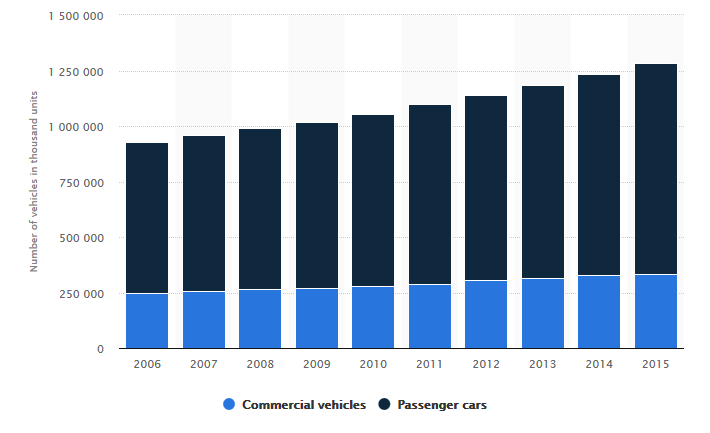
\includegraphics[width=14cm]{liczbaPojazdowSwiat}
 \caption{Liczba pojazdów na świecie}
 \label{fig:liczbaPojazdowSwiat}
\end{figure} \noindent
W Polsce wzrost liczby pojazdów w latach 2006 - 2015 był jeszcze większy \cite{liczbaPojazdowPolska}. W 2006 roku według GUS w Polsce było zarejestrowanych 13,4 miliona samochodów osobowych. W 2015 roku ich liczba wynosiła już 20,7 miliona, co wyznacza 5 procentowy roczny wzrost liczby pojazdów.
Najbardziej zatłoczonym polskim miastem jest Łódź. Według rankingu firmy \textit{TomTom } Łódź zajmuje bardzo wysokie 5 miejsce na świecie i 1 w Europie pod względem zatłoczenia dróg \cite{rankingTomTom}. Oprócz Łodzi w pierwszej setce najbardziej zatłoczonych miast świata są inne polskie miasta: Lublin(34), Kraków(48), Warszawa(50), Wrocław(63), Poznań(69), Bydgoszcz(83). Zatory drogowe są jednak problem całej Europy. Spośród 100 najbardziej zatłoczonych miast świata aż 45 znajduje się w Europie. W 2008 roku Unia Europejska oszacowała, iż koszty zatłoczenia dróg kształtują się na poziomie $0,9\%-1,5\%$ PKB unijnego \cite{ue2008}. Następny raport z 2017 roku może napawać optymizmem, gdyż przedstawione w nim wyliczenia określiły jedynie $0,77\%$ straty całkowitego PKB wspólnoty \cite{ue2017}. Ten sam raport ocenia koszty zatorów komunikacyjnych w Polsce na poziomie $1,2\%$ polskiego PKB.
Problem zatorów komunikacyjnych jest trudny do rozwiązania na terenach zurbanizowanych, gdzie często brakuje przestrzeni do wybudowania dróg o większej przepustowości. Naturalnym rozwiązaniem wydaje się być wprowadzenie sygnalizacji świetlnych na zatłoczonych skrzyżowaniach. Niepodważalnie istotną kwestią jest wtedy optymalizacja ustawień sygnalizacji świetlnej. Praca jest poświęcona temu aspektowi.

\chapter{Cel i zakres pracy} \label{sec:cel_zakres_pracy}
Celem pracy jest przedstawienie metod uczenia maszynowego, których zadaniem będzie ustalenie strategii doboru faz świetlnych tak, aby zapewnić jak największy przepływ ruchu drogowego. W rozdziale \ref{chapter:reinforcement} przedstawiona zostanie metoda uczenia ze wzmocnieniem wykorzystana w optymalizacji sygnalizacji świetlnej. Rozdział \ref{chapter:makroskopowy_model_ruchu} opisuje przepływowy model ruchu pojazdów, który będzie obowiązywał w symulacjach drogowych. W rozdziale \ref{chapter:model_sieci_drog} przedstawiony zostanie model sieci dróg. Początkowy model będzie bardzo prosty z pominięciem większości aspektów. W każdej kolejnej sekcji rozdziału będzie stopniowo rozwijany. Rozdział \ref{chapter:envs} przedstawia środowiska symulacyjne dla których zostanie przeprowadzony proces optymalizacji sygnalizacji świetlnych. Ostatnie środowisko testowe w pracy przedstawia sieć dróg wokół kampusu B Politechniki Łódzkiej i to głównie na optymalizacji tego środowiska będzie skupiona uwaga. Wszystkie poprzednie sieci dróg są mniej skomplikowane i służą przedstawieniu modelu i procesu optymalizacji. Stworzony przez autora pracy został program symulujący ruch drogowy środowisk z rozdziału \ref{chapter:envs}. Specyfikacja technologiczna, wymagania i instrukcje uruchomienia programu zostały przedstawione w załączniku do pracy.


\chapter{Uczenie ze wzmocnieniem} \label{chapter:reinforcement}
\section{Kategorie uczenia maszynowego}
Uczenie maszynowe to dziedzina wchodząca w skład nauk zajmujących się sztuczną inteligencją\cite{ml_ai}. Samo uczenie maszynowe w najprostszym kształcie może być rozumiane jako dobór optymalnych parametrów na podstawie dostępnych danych. Uczenie maszynowe jest powszechnie dzielone na 3 kategorie nauki \cite{machineLearningClassification}.
\begin{enumerate}
	\item \textbf{Nadzorowane} \\
	Dane używane do uczenia nazywane są zbiorem treningowym. Każdy pojedynczy element zbioru treningowego ma informacje wejściowe oraz pewną pożądaną wartość wyjściową. W trakcie uczenia algorytm dopasowuje swoje parametry tak aby na podstawie danych wejściowych mógł przewidzieć wartość wyjściową. Przykładami uczenia nadzorowanego jest np. rozpoznawanie tekstu pisanego, detekcja obiektów na zdjęciach.
	\item \textbf{Nienadzorowane} \\
	Uczenie nienadzorowane różni się od nadzorowanego tym, że nie  są znane pożądane wartości wyjściowe. Celem nauki jest przydzielenie elementów do odpowiednich klas. Odbywa się to na podstawie podobieństw poszczególnych elementów. Przykładem uczenia nienadzorowanego może być np. klasyfikacja gatunków drzew na podstawie danych jedynie o ich wysokościach i szerokości korony drzew.
	\item \textbf{Wzmocnione} \\
	W środowisku uczenia ze wzmocnieniem istnieje agent(lub kilku), który jest odpowiedzialny za podejmowanie pewnych akcji. Każda akcja ma wpływ na zmianę stanu środowiska, które w międzyczasie zwraca agentowi nagrodę. Uczenie ze wzmocnieniem jest oparte o strategie doboru akcji maksymalizujących skumulowaną wartość nagród.
\end{enumerate}
Przedstawiony w pracy problem optymalizacji sygnalizacji świetlnej zostanie rozważony w kontekście uczenia ze wzmocnieniem.
\section{Uczenie ze wzmocnieniem} \label{sec:reincorcement}
Schemat uczenia ze wzmocnieniem składa się z następujących elementów:
\begin{enumerate}
	\item \textbf{Agent} jest odpowiedzialny za podejmowanie decyzji odnośnie wykonania pewnych akcji. Ma on wiedzę na temat obecnego stanu środowiska i otrzymuje w każdym kroku czasowym sygnał nagrody. Agentów może być więcej niż jeden. Wtedy mówimy, że system jest wieloagentowy. Akcje podjęte przez agenta wpływają na zmianę stanu środowiska.
	\item \textbf{Środowisko} jest przestrzenią posiadającą dynamiczny stan widoczny dla agenta. Chociaż to agent podejmuje akcje, to środowisko ma zdefiniowany model zmiany stanu. Model zmiany stanu może być stochastyczny oraz niewidoczny dla agenta. Oznacza to, że dwie te same akcje podjęte w tym samym stanie nie zawsze przyniosą identyczny następny stan. Innymi słowy agent nie może być stuprocentowo pewny rezultatów swoich akcji. Środowiska rozważane w rozdziale \ref{chapter:envs} są jednak w pełni deterministyczne.
	\item \textbf{Strategia} definiuje sposób doboru akcji przez agenta. Jest to funkcja, która przyjmuje stan środowiska i zwraca akcje, która powinna być przeprowadzona. 
	\item \textbf{Sygnał nagrody} jest liczbą rzeczywistą, którą otrzymuje agent po podjęciu akcji. Określa ona jak dużą natychmiastową korzyść przyniosła ta akcja. Wartości nagród są czynnikiem wpływającym na zmianę strategii, gdyż zadaniem agenta jest maksymalizacja nagród. Wartość nagród zatem definiuje, które zdarzenia są dobre, a które złe dla agenta. Biologicznym odpowiednikiem dodatniej nagrody jest przyjemność, a ujemnej - ból \cite{berridge2000reward}. 
	\item \textbf{Funkcja wartości} zwraca wartość stanu czyli oczekiwaną sumę nagród, które agent otrzyma w przyszłości będąc aktualnie w tym stanie. 
\end{enumerate}
\begin{figure}[H]
	\centering
	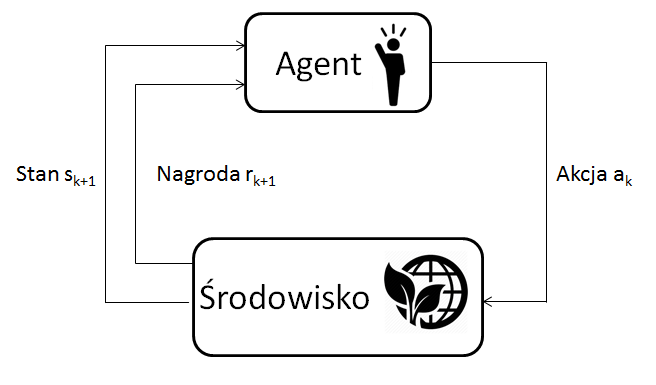
\includegraphics[width=14cm]{agent-srodowisko}
	\caption{Interakcje pomiędzy agentem a środowiskiem.}
	\label{fig:agent-srodowisko}
\end{figure}
\newpage
\subsection*{Proces Markowa}
Algorytmy uczenia ze wzmocnieniem zazwyczaj stosuje się do rozwiązywania problemu procesu decyzyjnego Markowa \cite{reinforcementBook}. Sam \textbf{proces decyzyjny Markowa} jest zdefiniowany jako uporządkowana czwórka $(S,A,P^a,R^a)$, gdzie:
\begin{enumerate}
	\item $S$ to zbiór wszystkich stanów.
	\item $A$ to zbiór akcji. Notacją $A_s$ oznaczane są możliwe akcje do podjęcia w stanie $s$.
	\item $P^a(s,s')=Pr(s_{t+1}=s'|s_t=s,a_t=a)$ to prawdopodobieństwo, że akcja $a$ wykonana w stanie $s$ w chwili $t$ doprowadzi do stanu $s'$ w chwili $t+1$.
	\item $R^a(s,s')$ to oczekiwana nagroda otrzymana w wyniku akcji podjętej w stanie $s$ prowadzącej do stanu $s'$. W dalszych rozważaniach $R_k$ będzie oznaczało nagrodę za akcję podjętą w chwili $k$.
\end{enumerate}
\subsection*{Problem procesu Markowa}
Problemem procesu decyzyjnego Markowa jest odnalezienie optymalnej strategii. Strategia określona jest jako funkcja $\pi(s)$ przyjmująca jako argument stan, a zwracająca podejmowaną akcję. Celem optymalizacji jest odnalezienie strategii maksymalizującej następującą wartość:
\[
G=\sum_{k=0}^{K} \gamma^k R_{k}. \addtag \label{eq:Markov_maximize}
\]
Chociaż we wzorze \myref{eq:Markov_maximize} nie ma strategii $\pi(s)$, to wpływa ona na otrzymywane nagrody $R_{k}$, gdyż określa podejmowane akcje. Parametr $\gamma \in [0,1]$ jest współczynnikiem dyskontowym. 
\subsubsection*{Idea dyskontowania}
Idea dyskontowania nagród została zaczerpnięta z rachunku finansowego. Odległe w czasie przychody powinny być traktowane jako mniej wartościowe niż te, które są natychmiastowe. Z tego powodu wartość przyszłych przychodów z chwili $k$ są wymnażane $k$-krotnie przez współczynnik dyskontowy, aby je porównać z przychodami z chwili obecnej. Podobnie powinny być liczone nagrody, co uwzględnia wzór \myref{eq:Markov_maximize}. Im wartość $\gamma$ jest bliższa 0 tym bardziej istotne są początkowe nagrody. Dla $\gamma=1$ wszystkie nagrody są równie istotne - bez względu na czas ich otrzymania.\\
\subsubsection*{Wartość stanu}
Analogicznie do (\ref{eq:Markov_maximize}) jest ustalona funkcja wartości stanu. Wartość stanu $s$, który miał miejsce w chwili $t$ jest określona jako:
\[
G_t=\sum_{k=t}^{K} \gamma^k R_{k}=R_{t}+\gamma R_{t+1}+\gamma^{2} R_{t+2}+...+\gamma^{K}R_K. \addtag \label{eq:Markov_state_value_G}
\]
\subsubsection*{Przykład obliczeniowy}
Zostanie przedstawiony teraz przykład obliczeniowy. Agent podejmuje decyzje na których podstawie otrzymuje ciąg  nagród $R_0=0, R_1=2,R_2=6,R_3=-1,R_4=2,R_5=1$. Czynnik dyskontujący $\gamma$ jest równy 0,9. Jaka jest wartość sumy zdyskontowanych nagród $G$ oraz kolejnych stanów tj. $G_1,G_2,G_3,G_4,G_5$?\\
\begin{figure}[H]
	\centering
	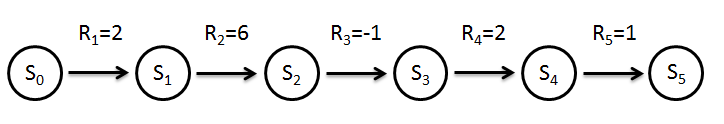
\includegraphics[width=14cm]{rewards-graph}
	\caption{Ciąg nagród i stanów.}
	\label{fig:agent-srodowisko}
\end{figure}\noindent
Najłatwiej obliczenia rozpocząć od $G_5$ i zakończyć na $G_1$.
\[G_5=R_5.  \addtag\]
Wzór \myref{eq:Markov_state_value_G} można przekształcić do następującej postaci dla $t \in \{1,2,3,4\}$:
\[G_{t}=R_{t}+\gamma G_{t+1} \label{eq:G_reccurential}. \addtag \]\\
$G_5=R_5=1.$\\
$G_4=R_4+\gamma G_{5}=\;\;2+0,9\cdot 1=2,9.$\\
$G_3=R_3+\gamma G_{4}=\!-1+0,9\cdot2.9=1,61.$\\
$G_2=R_2+\gamma G_{3}=\;\;6+0,9\cdot1,61 \approx 7,45.$\\
$G_1=R_1+\gamma G_{2}=\;\;2+0,9\cdot 7,45 \approx 8,70.$\\
$G\;\,=R_0+\gamma G_{1}=\;\;0+0,9\cdot 8,70 \approx 7,83.$\\

\section{Nomenklatura uczenia ze wzmocnieniem}
\subsection*{Algorytmy model-free i model-based}
Algorytmami nie wymagającymi modelu środowiska (model-free) nazywane są algorytmy, które nie wykorzystują prawdopodobieństw określających możliwe konsekwencje akcji (punkt 3 wcześniej opisanego procesu Markowa). Algorytmy wymagające modelu środowiska (model-based) z kolei bazują na nich \cite{reinforcementBook}.
\subsection*{Epizody treningowe i testowe}
Jako epizod rozumiana jest pełna symulacja środowiska. Środowiska epizodyczne posiadają pewien warunek zakończenia symulacji (np. limit czasowy, osiągnięcie pewnego celu). Epizody treningowe mają na celu jedynie generowanie danych do nauki agentów. Mogą one być przeprowadzane wedle dowolnej strategii ustalonej przez programistę. Z kolei epizody testowe mają na celu przetestować działanie obecnie wyuczonej strategii.
\subsection*{Optimal policy i behaviour policy}
Pierwszy termin - \emph{optimal policy} odnosi się do strategii zachłannej, czyli podejmowania jedynie najlepszych możliwych akcji wedle dotychczas wyuczonej strategii $\pi$. Epizody testowe są zawsze przeprowadzane według zachłannej strategii. Kolejny termin - \emph{behaviour policy} odnosi się do strategii zachowania podczas epizodów treningowych. Sposób wyboru akcji podczas treningu jest bezpośrednio związany z poniższym rozważaniem.
\subsection*{Exploration or Exploitation (eksploracja czy eksploatacja)}
Exploration or Exploitation jest bardzo często pojawiającym się terminem w artykułach tematyki uczenia ze wzmocnieniem\cite{exploration_or_exploitation}, gdyż dotyczy on właściwie każdego problemu uczenia ze wzmocnieniem. Termin ten odnosi się do dylematu jakie agent powinien wybierać akcje podczas treningu. Agent może wybierać akcje losowe (eksploracja) albo najlepsze według wyuczonej polityki (zachłanne - eksploatujące). Mogłoby się wydawać, że pełna eksploracja jest dobrym rozwiązaniem podczas epizodów treningowych. Zazwyczaj tak jednak nie jest. Podejmowanie jedynie losowych akcji może prowadzić środowisko do stanów, które nie będą miały miejsca w epizodach testowych. Powstaje przez to szum informacyjny, który zaburza i spowalnia uczenie. Może też dojść do odwrotnej sytuacji. Akcje w pełni losowe mogą skutkować nie zbadaniem pewnych stanów. Doskonałym środowiskiem przedstawiającym ten problem jest `MountainCar-v0` biblioteki OpenAi Gym \cite{openai}. Przedstawia ono pojazd w dolinie, którego celem jest podjechanie pod górkę z flagą. Nie może tego zrobić jedynie jadąc w prawo. Pojazd musi się rozpędzić wjeżdżając pierw na pagórek z lewej strony. W pełni losowe akcje powodują zatrzymanie pojazdu w dolinie. Nie zostaną zbadane wtedy stany w których pojazd jest na zboczu góry. Agent musi podjąć szereg zarówno zachłannych jak i losowych akcji. Doprowadzą one pojazd wyżej, w przeciwnym razie wiele stanów nigdy nie pojawi się w epizodach treningowych.
\begin{figure}[H]
	\centering
	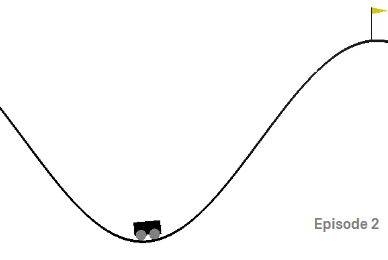
\includegraphics[width=10cm]{images/mountain_car}
	\caption{Środowisko MountainCar-v0 biblioteki OpenAi Gym }
	\label{fig:mountain-ca}
\end{figure}\noindent
\subsection*{Strategia $\mathbf{\epsilon}$ - zachłanna}
Parametrem wyznaczającym proporcje akcji eksploracyjnych i eksploatacyjnych w trakcie epizodów treningowych oznacza się $\epsilon \in [0,1]$. Zanim zostanie podjęta akcja losowana jest pewna liczba $u$ z przedziału $[0,1]$ wedle rozkładu jednostajnego. Jeżeli $u<\epsilon$ agent podejmuje losową akcję (eksploracja). W przeciwnym przypadku gdy $u \geq \epsilon$ podejmowana jest najlepsza akcja wedle dotychczas wyuczonej strategii (eksploatacja). Zazwyczaj na początku nauki $\epsilon=1$, aby za pomocą losowych akcji dokonać eksploracji środowiska. W dalszych etapach często opłacalnym jest zmniejszenie wartości $\epsilon$ \cite{epsilon_decay}.

\section{Metoda Q-learning}
Q learning jest prostym algorytmem uczenia ze wzmocnieniem rozwiązujący problem Markowa \cite{watkins}. Jest to algorytm nie wymagający modelu środowiska (model-free). Wykazane zostało\cite{q_zbieznosc}, że dla skończonych procesów Markowa algorytm Q learning odnajduje strategię, która jest optymalna w sensie maksymalizacji wartości oczekiwanej nagród \myref{eq:Markov_maximize}. Nazwa metody wzięła się od wartości $Q(s,a)$, która określa opłacalność podjęcia akcji $a$ w stanie $s$ \cite{nazwa_q}. Algorytm przedstawiony jest poniższym pseudokodem.
\begin{enumerate}
	\item Zainicjuj słownik
	$Q(s,a)$ przypisany do jednego agenta. Jego wartości określają opłacalność wyboru akcji $a$ w stanie $s$.
	\item Zasymuluj $\epsilon$ - zachłanny epizod treningowy. Obserwuj jakie zostały podjęte akcje $a$ w stanie $s$ i do jakiego stanu $s'$ one doprowadziły oraz jaka została przyznana nagroda $r$.
	\item Dla każdej obserwacji $(s,a,s',r)$, która pojawiła się w epizodzie przypisz nowe wartości $Q(s,a)$:
	\[Q(s,a) \leftarrow (1-\alpha)Q(s,a) + \alpha [r + \gamma \max_{a' \in A_{s'}} Q(s',a')]. \addtag \label{eq:q_rozwoj} \]
\end{enumerate}
\subsubsection{Zalety} 
Warto zauważyć następujące zalety metody Q-learningu:
\begin{enumerate}
	\item Brak potrzeby wiedzy na tematu modelu środowiska - tj. rozkładu prawdopodobieństwa konsekwencji akcji.
	\item Nie wymaga często nierealnego założenia, iż stan środowiska może zostać sztywno ustalony przez programistę. Wymagana jest jedynie możliwość przeprowadzenia pełnych epizodów, co jest nieporównywalnie słabszym założeniem.
	\item W przypadku dobrze wybranego parametru $\epsilon$ dostarczane są adekwatne dane do nauki agenta. Czas treningowy jest poświęcony dla stanów, które są często odwiedzane. Z kolei te, które nie pojawiają się prawie wcale - nie marnują czasu w procesie nauki.
	\item Daje pewność maksymalizacji zdyskontowanej wartości oczekiwanej nagród.
\end{enumerate}
\subsection*{Skalowanie metody}
Dla bardziej złożonych środowisk - z dużą przestrzenią stanu i akcji powyższy algorytm często okazuje się niewystarczający \cite{q_zlozony_env}. Gdy przestrzeń stanów jest bardzo duża, ograniczenia czasowe mogą nie pozwolić na eksplorację każdego stanu, co skutkuje dużą liczbą wartości $Q(s,a)$ niezmienionych od momentu inicjacji słownika. Jako przykład problemu niech stanem środowiska będzie kolejka na 3 odcinkach przed skrzyżowaniem. Wtedy dwa bardzo podobne stany, na pozór wręcz identyczne $[3,22,72]$ oraz $[3,22,73]$ są od siebie różne i w trakcie treningu należy prześledzić oddzielnie każdy z tych stanów. Zakładając, że wartości każdej zmiennej należą do zbioru $\{0,1,...,100\}$ liczność przestrzeni stanu jest równa aż 1 000 000. Lepiej skalującym rozwiązaniem jest zastosowanie sieci neuronowych zamiast tablic. Zostanie ono przedstawione w następnej sekcji.

\section{Metoda Q-learning z użyciem sieci neuronowej} \label{learning:DQN_single_agent}
Rozwiązaniem problemu skalowalności Q-learningu jest zastosowanie sieci neuronowych do aproksymacji wartości $Q$ zamiast słowników. Sieć neuronowa tworzy funkcje rzeczywistą, która ma za zadanie aproksymację wartości $Q$. W przeciwieństwie do słowników funkcja ta może przybliżać też wartości $Q(s,a)$ dla stanów i akcji, które nie pojawiły się w trakcie symulacji treningowych. Algorytm uczenia jest wtedy następujący:
\begin{enumerate}
	\item Stwórz sieć neuronową dla wartości $Q$ dla każdego agenta (chyba, że już została wcześniej utworzona).
	\item Zasymuluj $\epsilon$ - zachłanne epizody treningowe. Obserwuj jakie zostały podjęte przez agentów akcje $a$ w stanie $s$ i do jakiego stanu $s'$ one doprowadziły oraz jaka została przyznana nagroda $r$.
	\item Trenuj sieć neuronową każdego agenta na podstawie danych wygenerowanych w trakcie symulacji treningowych.
	\item Jeśli nie jest spełniony warunek stopu zacznij nową iterację wracając do kroku 2, w przeciwnym razie zakończ algorytm.
\end{enumerate}
Krok 3 powyższego algorytmu wymaga dokładnego wyjaśnienia.
\subsection{Wygenerowane dane podczas symulacji treningowych}
Dla każdej z obserwacji $(s,a^*,s',r)$ wygenerowany zostaje element $(\textbf{x},\textbf{y})$, gdzie $\textbf{x}$ jest wektorem utworzonym na podstawie stanu $s$ i nazywany będzie \textbf{sygnałem wejściowym}. Powinien on zawierać jedynie istotne dla agenta informacje na temat stanu środowiska. Z kolei $\textbf{y}$ jest wektorem przedstawiającym wartość $Q$ dla rozważanego stanu $s$ i wszystkich możliwych akcji $a$. Nazywany on będzie \textbf{sygnałem wyjściowym}. Dla akcji z obserwacji, czyli $a=a^*$ wartość $y[a]$ jest wyliczana ze znanego już wcześniej wzoru \myref{eq:q_rozwoj}:
\[ y[a]=(1-\alpha)Q(s,a) + \alpha [r + \gamma \max_{a' \in A'} Q(s',a')]. \addtag \]
Gdzie wartości $Q(s,a)$,$Q(s',a')$ są aproksymacjami uzyskanymi przez sieć neuronową. \newline \newline Dla pozostałych akcji $a \neq a^*$ wartość $y[a]$ jest uzyskana z dotychczasowej aproksymacji sieci neuronowej dla stanu $s$ i akcji $a$. Tak utworzone pary $(\textbf{x},\textbf{y})$ ze wszystkich obserwacji tworzą zbiór na podstawie których przebiega trening.


\subsection{Trening sieci neuronowej}
Wygenerowany wcześniej zbiór jest dzielony na dwie części - treningową i walidacyjną. Nie wgłębiając się szczegółowo w strukturę sieci neuronowej - posiada ona parametry nazywane wagami. Wagi te definiują funkcję $f$, która jako argument przyjmuje sygnał wejściowy $\mathbf{x_{i}}$. Są one zmieniane w trakcie treningu tak aby wartości funkcji $f(\mathbf{x_i})$ najlepiej przybliżały wartości sygnału wyjściowego $\mathbf{y_i}$. Oceną jakości aproksymacji jest wartość funkcji straty. Dla wszystkich sieci neuronowych w tej pracy funkcją straty będzie błąd średniokwadratowy dany wzorem: 
\[\
\frac{1}{n}\sum_{i=1}^{n} (f(\mathbf{x_i})-\mathbf{y_i})^2. \addtag
\]
Sposoby zmian wag są zazwyczaj oparte na metodach gradientowych \cite{overview_optimizers}. W cytowanym artykule znajduje się przegląd najczęściej używanych metod gradientowych. Warto zauważyć, że zmiana wag jest podyktowana poprzez elementy zbioru treningowego, a nie zbioru walidacyjnego. Jednym z przeznaczeń zbioru walidacyjnego jest sprawdzenie jak dobrze sieć neuronowa prognozuje wartości z poza zbioru treningowego(ekstrapolacja). Częstą praktyką jest przerwanie trenowania sieci neuronowej(optymalizacji wag) w chwili gdy dla danych zbioru walidacyjnego otrzymuje się coraz gorsze aproksymacje. Jest to znak, że sieć neuronowa przestaje generalizować, a zaczyna zapamiętywać wartości treningowe. Jest to niepożądane zachowanie znane jako nadmierne dopasowanie. 
\subsection{Modyfikacja wzoru Q dla fazy żółtych świateł} \label{sec:q_mod}
W rozdziale \ref{chapter:model_sieci_drog} przedstawione zostaną środowiska sieci dróg oraz model działania sygnalizacji świetlnych. W kontekście algorytmu Q-learningu rozważony zostanie przypadek, gdy faza sygnalizacji świetlnej przypisanej do pewnego agenta to `żółte`. Agent wtedy jest zobowiązany do podjęcia akcji `żółte`. Niepotrzebne jest zatem wyliczanie wartości Q dla tej wymuszonej akcji. Aby ustrzec sieć neuronową od aproksymacji nieistotnych wartości zostaną podjęte następujące kroki. Jeśli dana jest wiedza na temat długości fazy żółtych świateł należy zastąpić wzór \myref{eq:q_rozwoj} poniższymi formułami. Niech faza żółtych świateł trwa $k$ interwałów czasowych, wtedy dla akcji $a$ zmiany obecnej fazy:
\[Q(s,a) \leftarrow  (1-\alpha)Q(s,a) + \alpha [\gamma^{k} r + \gamma^{k+1} \max_{a' \in A_{s'}} Q(s',a')]. \addtag \label{eq:Q_DQN_II} \]
Dla akcji $a$ utrzymania obecnej fazy:
\[Q(s,a) \leftarrow (1-\alpha)Q(s,a) + \alpha [r + \gamma \max_{a' \in A'} Q(s',a')]. \addtag \label{eq:Q_DQN_I} \]
\chapter{Makroskopowy model ruchu} \label{chapter:makroskopowy_model_ruchu}
\section{Klasyfikacja modeli ruchu drogowego}
Modele ruchu drogowego mają na celu ukazanie rzeczywistego przepływu pojazdów w sposób czysto matematyczny. Ważnym kryterium doboru modelu jest przystępność jego implementacji informatycznej. Powszechnie klasyfikuje się 3 podejścia modelowe dla omawianego problemu \cite{CompareModels} - makroskopowy, mezoskopowy oraz mikroskopowy. Czasem \cite{multilevel} wyróżnia się także czwarte podejście - submikroskopowe. Jest to podział ze względu na poziom modelu. Najniższy poziom i najbardziej dokładny model gwarantuje podejście mikroskopowe. Rozważa ono pojazdy indywidualnie w czasoprzestrzeni. Przyspieszenie pojazdu jest wyliczane na podstawie dynamiki(prędkości, przyspieszenia) i pozycji pojazdu bezpośrednio przed nim. Model mezoskopowy zapewnia indywidualne rozróżnienie pojazdów, jednak ich zachowanie jest wyliczane na danych zagregowanych \cite{mesoscopic}. Przykładowo pojazdy są podzielone na grupy podróżujące od pewnego punktu startowego do punktu końcowego. Inne modele mezoskopowe wyliczają dynamikę ruchu na podstawie aktualnego zatłoczenia drogi \cite{mesoscopic2}. Poziom mezoskopowy jest obliczeniowo bardziej opłacalny od mikroskopowego.
Wiele symulatorów stosujących model mezoskopowy oferuje symulację w czasie rzeczywistym dla sieci dróg całego miasta\cite{vu2017high}. Ideą modelu makroskopowego jest traktowanie ruchu ulicznego identycznie jak ruchu cieczy lub gazów. Po raz pierwszy w roku 1956 M. J. Lighthill i G. B. Whitham \cite{lwr} przedstawili pomysł przyrównania ruchu ulicznego na zatłoczonych drogach do przepływu wody w rzekach. Z tego powodu nie uznajemy w nim pojazdów jako niepodzielne jednostki. Pojazd można przyrównać do pewnej ilości wody w rzece.
Jest to najmniej kosztowny obliczeniowo model. Właśnie w modelu makroskopowym zostało stworzone środowisko symulacyjne i dlatego zostanie on dokładnie przedstawiony w tym rozdziale.

\section{Wstęp}
Jako zmienną stanu makroskopowego modelu ruchu zazwyczaj wybierana jest gęstość ruchu \cite{gottlich,CompareModels}. Formalnie gęstość można rozumieć jako czynnik definiujący dynamikę ruchu. Im większa jest gęstość tym mniejsza prędkość ruchu. Gęstość ruchu \cite{helbing2001master} jest przedstawiona jako iloraz liczby pojazdów znajdujących się na pewnym odcinku i długości tego odcinka drogi. Prawidłowe jest także uznanie liczby pojazdów na pojedynczym odcinku drogi jako zmienną stanu. Należy jednak pamiętać, że pojazdy w ruchu makroskopowym nie są nierozłączną jednostką. Pojazd w analogii do przepływu wody w rzece jest pewną jednostką objętości wody. Wielokrotnie w symulacjach zdarza się, że na odcinku jest zatem niecałkowita liczba pojazdów.

\section{Rozwój gęstości ruchu na drodze}
Makroskopowy model ruchu jest oparty o równanie różniczkowe (\ref{eq:main_diff_eq}) wraz z warunkiem początkowym (\ref{eq:p_init_eq}) \cite{gottlich}. W analogii do przepływu wody w rzece gęstość ruchu można utożsamiać z polem powierzchni przekroju poprzecznego rzeki, co dla stałej szerokości rzeki - upraszcza się do wysokości wody w rzece.   \\Dla ustalonej pojedynczej drogi zmianę gęstości ruchu definiuje następujący układ równań:\\
\begin{numcases}{}
   p(x,0)=p_{0}(x) \label{eq:p_init_eq}
   \\
   \frac{\partial p(x,t)}{\partial t}+\frac{\partial f(p(x,t))}{\partial x}=0 \label{eq:main_diff_eq}
\end{numcases}
Gdzie $p(x,t)$ to gęstość ruchu w punkcie $x$ i czasie $t$. Wartość funkcji gęstości należy do przedziału $[0,p^{max}]$.\\
Równanie (\ref{eq:p_init_eq}) zakłada istnienie pewnej z góry nałożonej początkowej gęstości drogi $p_0(x)$.
Równanie (\ref{eq:main_diff_eq}) określa
wedle założeń modelu makroskopowego rozwój gęstości ruchu na drodze. Funkcja płynności ruchu $f$ powinna być wklęsła \cite{gottlich,lwr}. 
%W przedstawionym w tej pracy modelu funkcja ma następującą definicję:
%\begin{numcases}{f(p)=}
%   \lambda p & \text{dla } $p\in[0,p^{*}]$\\
%   \lambda \cdot (2p^{*}-p) & \text{dla } $p\in(p^{*},p^{max}]$ 
%\end{numcases}
%Gdzie $\lambda$ jest stałym parametrem funkcji trójkątnej oraz $p^*=\frac{1}{2}p^{max}$.
\section{CTM - Cell Transmission Model} \label{sec:CTM}
\subsection{Wprowadzenie}
W tym rozdziale zostanie przedstawiony model CTM będący dyskretyzacją pierwotnego modelu makroskopowego przepływu \cite{lwr}. Jego zmienną stanu jest liczba pojazdów. Model został przedstawiony przez Carlosa Daganzo w \cite{CTM}. Pozycja jest podstawą wyliczeń w tym rozdziale.
\subsubsection*{Siatka czasowa i przestrzenna drogi}
Dyskretny charakter modelu CTM obliguje do określenia siatki czasowej i przestrzennej drogi. Dla par czasu i odcinków należących do tych dwóch siatek będą określane zmienne stanu. \\ \\ \textbf{Siatka czasowa} jest zdefiniowana jako skończony ciąg liczb naturalnych:
\[(0,1,...,T). \addtag \]
Następnie zdefiniowana zostanie siatka przestrzenna drogi e. Ustalona droga e to odcinek $[0,L]$. Zostaje ona podzielona na $L$ odcinków o równej długości. \textbf{Siatka przestrzenna} drogi to ciąg odcinków:
\[([0,1),[1,2),...,[L-1,L] ). \addtag \]

\subsection{Model CTM dla pojedynczej drogi}
\subsection*{Przepływ pojazdów na drodze}
Niech dana będzie droga $e$ i pewien odcinek $j$ na tej drodze. Zmienna stanu w modelu CTM jest oznaczana jako $x_j(t)$ i określa ona liczbę pojazdów na odcinku $j$ w chwili t.
Przepływ pojazdów opiera się o założeniu, iż przy braku zatorów pojazdy pokonują w jednym interwale czasowym jeden odcinek drogi. Przykładowy przepływ jest następujący:
\begin{figure}[H]
	\centering
	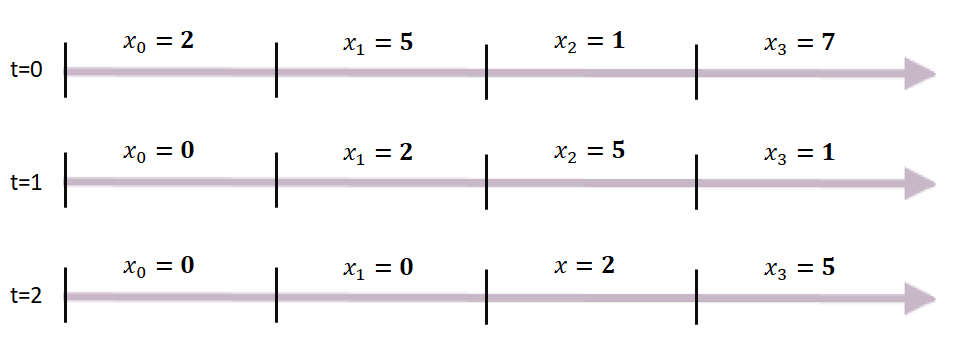
\includegraphics[width=14cm]{images/CTM_flow_example}
	\caption{Przykładowy przepływ bez zatorów w modelu CTM}
	\label{fig:CTM_flow_example}
\end{figure} \noindent
Łatwo zauważyć, że w tym przypadku
\[ x_{j+1}(t+1)=x_j(t). \addtag \]
\subsubsection*{Wprowadzenie zatorów}
Poprzedni przykład ruchu pojazdów opierał się o założenie, iż wszystkie pojazdy przemieszczają się o jeden odcinek w jednym interwale czasowym. Często jednak część pojazdów będzie musiała pozostać na dotychczasowym odcinku z powodu zbyt dużego natężenia ruchu. Taka sytuacja będzie nazywana \textbf{zatorem}. Model CTM opiera się o następujące parametry definiujące sposób formowania się zatorów:
\begin{itemize}
	\item $N_j(t)$ - maksymalna liczba pojazdów, które mogą znajdować się na odcinku $j$ w chwili $t$.
	\item $V_j(t)$ - maksymalna liczba pojazdów, które mogą napłynąć do odcinka $j$ w momencie $t+1$.
\end{itemize}
Rozwój zmiennej stanu jest zadany poprzez następujące równanie:
\[x_j(t+1)=x_j(t)+y_j(t)-y_{j+1}(t). \addtag \]
Gdzie:
\begin{itemize}
	\item $x_j(t+1)$ to liczba pojazdów na odcinku $j$ w chwili $t+1$.
	\item $x_j(t)$ to liczba pojazdów na odcinku $j$ w chwili $t$.
	\item $y_j(t)$ to liczba pojazdów napływających do odcinka $j$ w chwili $t+1$.
	\item $y_{j+1}(t)$ to liczba pojazdów napływających do odcinka $j+1$ w chwili $t+1$. Jest to zatem także liczba pojazdów opuszczających odcinek $j$ w interwale $[t,t+1)$.
\end{itemize}
\textbf{Przepływ pojazdów} $y_j(t)$ w modelu CTM jest zdefiniowany jako minimum z następujących trzech wartości:
\begin{itemize}
	\item $ x_{j-1}(t) $ - liczba pojazdów na poprzedzającym odcinku (tj. $j-1$).
	\item $ V_i(t) $ - maksymalna liczba pojazdów, które mogą napłynąć do odcinka $i$ w chwili $t+1$.
	\item $ N_i(t)-x_j(t) $ - liczba wolnych miejsc na odcinku $j$ w chwili $t$.
\end{itemize}
Co wyraża się wzorem:
\[
y_j(t)=Min\{x_{j-1}(t),V_i(t),N_i(t)-x_i(t)\}. \addtag \label{eq_y_CTM}
\]

\subsection*{Źródło i ujście ruchu}
Powyższe wzory potrzebują ustaleń odnośnie źródła i ujścia ruchu. Bez nich wzór \myref{eq_y_CTM} nie ma sensu dla krańcowych odcinków $j=0$ oraz $j=L-1$. Dla ułatwienia pogrubione zostały ustalone w tej sekcji wartości zmiennych źródła i ujścia ruchu. \\ Źródło ruchu może być traktowane jako odcinek o indeksie $j=-1$. Jedyną wartością, która musi być ustalona dla źródła jest liczba pojazdów w nim, czyli $x_{j-1}(t)$. 
Ujście ruchu może być traktowane jako odcinek $i=L$. Istotne w kontekście wzoru \myref{eq_y_CTM} są następujące wartości:
\begin{itemize}
	\item $V_{L}(t)$ - liczba pojazdów, które mogą opuścić odcinek $L-1$ w chwili $t$. Ustalone jest, że jest to dowolna liczba, wtedy $\mathbf{V_{L}(t)=\infty}$.
	\item $N_{L}(t)$ - liczba pojazdów, które może pomieścić ujście. Ustalone jest, że $\mathbf{N_{L}(t)=\infty}$, gdyż ujście może zawierać nieograniczoną liczba pojazdów.
	\item $x_{L}(t)$ - liczba pojazdów w ujściu. Służy jako licznik pojazdów, które opuściły układ.
\end{itemize}
\subsubsection*{Przykład przepływu na pojedynczej drodze}
Zostają ustalone następujące parametry implementacji przykładowego modelu
\begin{itemize}
	\item $L=9$ - liczba odcinków drogi.
	\item $N_i(t)=15$ dla dowolnego $i,t$ - odcinki drogi mogą pomieścić maksymalnie 15 pojazdów.
	\item Maksymalne przepływy są następujące: \begin{numcases}{V_i(t)=}
	1 & \text{dla } $i=5, t\in \{0,...,7\}$ \\ 
	5 & \text{dla } $i=5, t\in \{7,...,20\}$ \\ 	
	4 & \text{dla pozostałych przypadków}
	\end{numcases}
\end{itemize}
Podsumowując powyższe parametry - droga posiada 9 odcinków (ponumerowanych od 0 do 8). Każdy odcinek może pomieścić maksymalnie 15 pojazdów. Maksymalny przepływ z jednego odcinka na drugi to 4. Jedynym wyjątkiem od tej zasady jest odcinek nr. 5. Początkowo może napływać na niego tylko po 1 pojeździe. Zmienia się to dopiero w chwili $t=7$ - by rozładować powstałe zatory ustalone zostaje, że może co interwał wjeżdżać 5 pojazdów na odcinek 5. Przeprowadzona zostanie symulacja przy warunku początkowym określającym liczebność pojazdów na poszczególnych odcinkach. Niech zatem $x_i(0)=3$ dla $i \in \{0,...,8\}$. Wtedy wyniki symulacji przestawia poniższa tabela.
\begin{figure}[H]
	\centering
	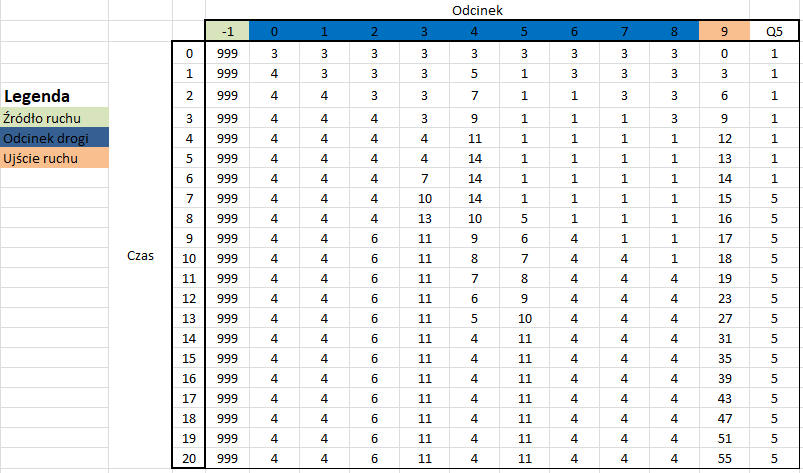
\includegraphics[width=14cm]{images/ctm_przyklad}
	\caption{Tabela liczby pojazdów}
	\label{fig:ctm_przyklad}\end{figure}
\subsection{Model CTM dla sieci dróg}
Poprzednio przedstawiony wariant modelu CTM określał przepływ jedynie dla jednej drogi. W tej sekcji zostanie rozważony przypadek modelu CTM dla sieci dróg. \textbf{Zbiór wszystkich odcinków} w środowisku będzie oznaczany jako $\Omega$. 
\subsubsection{Źródła ruchu}
W przypadku większej liczby dróg niż jedna należy rozważyć inne podejście do ustalenia źródeł ruchu. 
Dla każdego odcinka $j \in \Omega$ zostanie ustalona wartość $u_j(t)$ \textbf{napływu ze źródeł}. Określa ona ile pojazdów ze źródła może maksymalnie napłynąć do odcinka $j$ w chwili $t+1$. Dla odcinków $j$ do których nie wjeżdżają żadne pojazdy ze źródła ruchu wartość $u_j(t)$ jest równa 0. Wartości $u_j(t)$ tworzą \textbf{wektor źródła} ruchu:
\[\textbf{u}(t)=[u_0(t),...,u_{|\Omega-1|}(t)]. \addtag \]
Źródła ruchu są uwzględnione we wzorze na liczbę napływających pojazdów \myref{eq:y_with_zrodla}
\subsubsection{Ujścia ruchu}
Niech zbiór odcinków znajdujących się bezpośrednio przed punktami ujścia ruchu będzie oznaczony jako $\Omega_{out}$.
Zgodnie z poprzednimi założeniami pojazdy będące w chwili $t$ na odcinku bezpośrednio przed ujściem ruchu opuszczają układ w chwili $t+1$. Zostanie to uwzględnione we wzorze \myref{eq:ctm_rozwoj_x}.

\subsection{Przepływ pojazdów na skrzyżowaniu} \label{sec:CTM_skrz_przeplyw}
Wprowadzona zostanie modyfikacja funkcji $y_j(t)$ określającej liczbę pojazdów wjeżdżających na odcinek $j$ w chwili $t+1$. Do tej pory dotyczyła ona jedynie liczby pojazdów które napływają do odcinka $j$ z odcinka $j-1$. W przypadku sieci dróg należy rozważyć możliwość wjazdu z innych odcinków niż $j-1$. Niech zatem:
\[ y_{ij}(t)= Min\{p_{ij} x_{i}(t),V_j(t),N_j(t)-n_j(t)\}. \addtag \label{eq:y_skrz_no_lights}\]
określa liczbę pojazdów, które wjeżdżają z odcinka $i$ do odcinka $j$ w chwili $t+1$. Wartości $p_{ij}$ określają jaka część pojazdów z odcinka $i$ ma zamiar wjechać na odcinek $j$. Tworzą one macierz prawdopodobieństwa $\textbf{P}$, która została szczegółowo opisana w sekcji \myref{sec:macierz_prawd}. \\
Suma pojazdów opuszczających odcinek $i$ w chwili $t+1$ jest następująca:
\[y_{i*}(t)= \sum_{j\in \Omega / \{i\}} y_{ij}(t). \addtag \]
Z kolei napływ pojazdów do odcinka $j$ w chwili $t+1$ jest równy:
\[y_{*j}(t)= \sum_{i\in \Omega / \{j\}} y_{ij}(t)+u_j(t). \addtag \label{eq:y_with_zrodla}\]
Rozwój zmiennej stanu jest zdefiniowany przez równanie:
\begin{numcases}{x_j(t+1)=}
y_{*j}(t) &  dla $j \in \Omega_{out}$ \label{eq:ctm_rozwoj_x} \\
x_j(t)+y_{*j}(t)-y_{j*}(t) & dla $j \notin \Omega_{out}$ \label{eq:ctm_rozwoj_x_ujscie}
\end{numcases}
Dla przypomnienia wartości z powyższego równania oznaczają:
\begin{itemize}
	\item $x_j(t+1)$ - liczba pojazdów na odcinku $j$ w chwili $t+1.$
	\item $x_j(t)$ - liczba pojazdów na odcinku $j$ w chwili $t$.
	\item  $y_{*j}(t)$ - liczba pojazdów napływających do odcinka $j$ w chwili $t+1$.
	\item  $y_{j*}(t)$ liczba pojazdów opuszczających odcinek $j$ w chwili $t+1$.
\end{itemize}

\subsubsection{Przykład}
\begin{figure}[H]
	\centering
	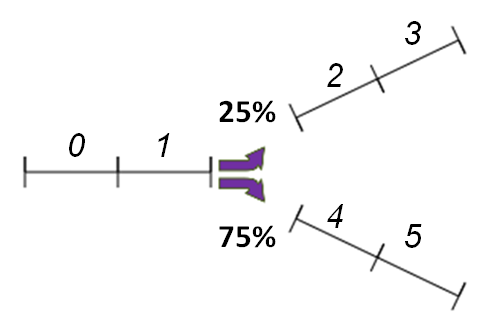
\includegraphics[width=13cm]{images/env_11_perc_italic}
	\caption{Numeracja odcinków sieci dróg}
	\label{fig:ctm_przyklad}\end{figure}
\def \xzero {\begin{bmatrix}
		7 \\ 4 \\ 3 \\ 0 \\ 1 \\ 5
\end{bmatrix}}
%\begin{figure}[H]
%	\centering
%	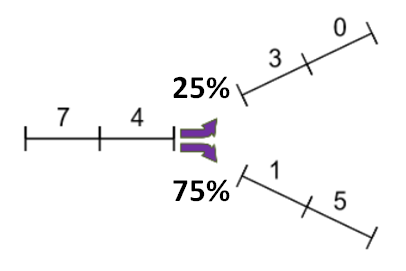
\includegraphics[width=14cm]{images/env_11_743015_procenty}
%	\caption{}
%	\label{fig:env_11_743015_procenty}\end{figure}
%\begin{tabular}{| c  | Sc |}
%	\hline
%	Numeracja odcinków   & Liczba pojazdów \\
%	\hline
%	\cincludegraphics[width=7cm]{images/env_11}  & \cincludegraphics[width=7cm]{images/env_11_743015_procenty} \\
%	\hline\end{tabular} \newline 
\def \A{
	\begin{bmatrix}
		0 & 0    & 0 & 0 & 0 & 0 \\
		1 & 0    & 0 & 0 & 0 & 0 \\
		0 & 0.25 & 0 & 0 & 0 & 0 \\
		0 & 0    & 1 & 0 & 0 & 0 \\
		0 & 0.75 & 0 & 0 & 0 & 0 \\
		0 & 0    & 0 & 0 & 1 & 0 
	\end{bmatrix}
}
Rozważony zostanie układ przedstawiony na powyższym obrazku. Na rozwidleniu dróg 75 procent pojazdów ma zamiar skręcić w prawo. Pozostałe 25 procent wybiera skręt w lewo. 
Wartości macierzy prawdopodobieństwa $\textbf{P}$ określają, jaka część pojazdów z odcinka zadanego przez kolumnę ma zamiar wjechać na odcinek zadany przez wiersz:
\def \Azero{
	\begin{bmatrix}
		\frac{4}{7} & 0    & 0 & 0 & 0 & 0 \\
		\frac{3}{7} & 0    & 0 & 0 & 0 & 0 \\
		0 & 0.25 & 0 & 0 & 0 & 0 \\
		0 & 0    & 1 & 0 & 0 & 0 \\
		0 & 0.75 & 0 & 0 & 0 & 0 \\
		0 & 0    & 0 & 0 & 1 & 0 
	\end{bmatrix}
} 
\def \P {\begin{bmatrix}
		0 & 0 & 0 & 0 & 0 & 0 \\
		1 & 0 & 0 & 0 & 0 & 0 \\
		0 & 0.25 & 0 & 0 & 0 & 0 \\
		0 & 0 & 1 & 0 & 0 & 0 \\
		0 & 0.75 & 0 & 0 & 0 & 0 \\
		0 & 0 & 0 & 0 & 1 & 0 
\end{bmatrix}}
\[\textbf{P}=\P \addtag \label{eq:p_example_ctm} \]
\newpage
\noindent Początkowe liczby pojazdów na odcinkach są następujące:
\begin{table}[H]
\begin{center}
\begin{tabular}{| c  | Sc |}
	\hline
	Zapis   & Rysunek \\
	\hline
	\makecell{$x_0(0)=7$ \\ $x_1(0)=4$ \\ $x_2(0)=3$ \\ $x_3(0)=0$ \\ $x_4(0)=1$ \\ $x_5(0)=5$ }  & \cincludegraphics[width=7cm]{images/env_11_743015_procenty} \\
	\hline
\end{tabular}
\caption {Liczby pojazdów w chwili $t=0$} \label{tab:t_0_pojazdow}
\end{center}
\end{table}
Do sieci nie napływają żadne pojazdy, zatem wartości wektora źródła są równe 0 co jest zapisane jako $\textbf{u}(0)=\theta$.
Liczba pojazdów będąca na odcinku jest ograniczona przez $N_j(j)=7$ dla dowolnego odcinka $i$ oraz chwili $t$. Maksymalny przepływ pojazdów w jednym interwale to $V_j(t)=4$.
Na podstawie wzorów (\ref{eq:ctm_rozwoj_x},\ref{eq:ctm_rozwoj_x_ujscie}) zostają wyliczone liczby pojazdów dla chwili $t=1$:
%\begin{center}
%x_0(1)=x_0(0)+y_{*0}(0)-y_{0*}(0)=7+0-3=4. \\
%x_1(1)=x_1(0)+y_{*1}(0)-y_{1*}(0)=4+3-4=3. \\
%x_2(1)=x_2(0)+y_{*2}(0)-y_{2*}(0)=3+1-3=1. \\
%x_2(1)=x_2(0)+y_{*2}(0)-y_{2*}(0)=3+1-3=1. \\
%x_3(1)=y_{*3}(0)=3. \\
%x_4(1)=x_4(0)+y_{*4}(0)-y_{4*}(0)=3+3-3=3. \\
%x_5(1)=y_{*5}(0)=1.
%\end{center}
\[
x_0(1)=x_0(0)+y_{*0}(0)-y_{0*}(0)=7+0-3=4. \addtag
\]
\[
x_1(1)=x_1(0)+y_{*1}(0)-y_{1*}(0)=4+3-4=3. \addtag
\]
\[
x_2(1)=x_2(0)+y_{*2}(0)-y_{2*}(0)=3+1-3=1. \addtag
\]
\[
x_3(1)=y_{*3}(0)=3. \addtag
\]
\[
x_4(1)=x_4(0)+y_{*4}(0)-y_{4*}(0)=3+3-3=3. \addtag
\]
\[
x_5(1)=y_{*5}(0)=1. \addtag
\]
\newpage
Przepływ pojazdów został zwizualizowany w poniższej tabeli. \newline \newline
\def \xI{\begin{bmatrix}
		4 \\ 3 \\ 1 \\ 3 \\ 3 \\ 1
\end{bmatrix}}
\def \xzero{\begin{bmatrix}
		7 \\ 4 \\ 3 \\ 0 \\ 1 \\ 5
\end{bmatrix}}
\begin{table}[H]
\begin{center}
	\begin{tabular}{| c |  Sc |}
		\hline
		t   &  Podgląd środowiska \\
		\hline
		0 &
		\cincludegraphics[width=10cm]{images/env_11_743015_przeplyw} \\
		\hline 
		1 & \cincludegraphics[width=10cm]{images/env_11_431331_procenty} \\
		\hline 
	\end{tabular}
\end{center}
\caption {Przepływ pojazdów w interwale czasowym $[0,1]$} \label{tab:rozwoj_z_0_1}
\end{table}

\subsection{Przepływ pojazdów na skrzyżowaniu z sygnalizacją świetlną} \label{sec:CTM_sygnalizacja}
W tej sekcji przedstawiony zostanie przypadek przepływu na skrzyżowaniu posiadającym sygnalizację świetlną. Nie różni się on mocno od poprzednio omawianego modelu ruchu na skrzyżowaniu bez sygnalizacji świetlnej \myref{sec:CTM_skrz_przeplyw}. Jedyną różnicą jest zmiana wzoru \myref{eq:y_skrz_no_lights}. Zostanie on zastąpiony następującą formułą:
\[ y_{ij}(t)= Min\{p_{ij}s_{ij}(t) x_{i}(t),V_j(t),N_j(t)-n_j(t)\}. \addtag \label{eq:y_skrz_lights}\]
Gdzie: $s_{ij}(t)$ jest wartością określoną przez macierz sygnalizacji świetlnej $S[j,i]$, która została opisana w sekcji \myref{sec:sygnalizacja}.


\chapter{Model sieci dróg} \label{chapter:model_sieci_drog}
\section{Wstęp}
Ze względu na dużą złożoność końcowego modelu zostanie przedstawiony najpierw bardzo prosty, podstawowy model. W każdej kolejnej sekcji dodawane będą zmiany przybliżające do ostatecznej postaci. Jest to podejście pozwalające na proste przedstawienie modelu, który zawiera bardzo wiele aspektów m.in:
sygnalizacji świetlnej, wielu dróg, zatoru drogowego, źródła i ujścia ruchu. Zestawienie w jednej sekcji wszystkich tych kwestii byłoby bardzo przytłaczające. Numeracja odcinków sieci dróg zawsze zaczyna się od 0. Z tego powodu także numeracja wierszy oraz kolumn macierzy, czy też wektorów rozpoczyna się od 0.


\section{Wektor stanu drogi} \label{sec:wektor_stanu_drogi}
\textbf{Wektor stanu} jest strukturą przedstawiającą stan środowiska. Dla każdego odcinka drogi składuje on wartości zmiennych stanu. Zmienna stanu jest identyfikowana jako liczba pojazdów na danym odcinku drogi. 
\subsection*{Przykład} \label{subsec:example-single-road}
Niech będzie dana droga z wydzielonymi czterema odcinkami. Przykładowy wektor stanu takiego środowiska to
\[\textbf{x}(t)=\begin{bmatrix}
2 \\ 4 \\ 3 \\ 0
\end{bmatrix} \addtag \]
Zawiera on w sobie następujące informacje dla chwili t:
\begin{itemize}
	\item Są 2 pojazdy na zerowym odcinku
	\item Są 4 pojazdy na pierwszym odcinku
	\item Są 3 pojazdy na drugim odcinku
	\item Nie ma żadnego pojazdu na trzecim odcinku
\end{itemize}

\begin{figure}[H]
	\centering
	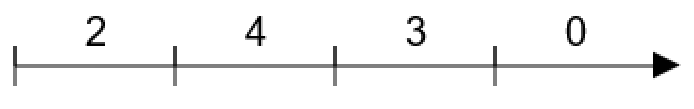
\includegraphics[width=14cm]{images/1_droga_4_odcinki}
	\caption{Droga z liczbą pojazdów na poszczególnych odcinkach}
	\label{fig:single_road}
\end{figure}
\section{Rozwój wektora stanu drogi i wprowadzenie macierzy systemu} \label{sec:macierz_systemu_def}
Formalnym wzorem definiującym rozwój wektora stanu jest:
\[\textbf{x}(t+1)=\textbf{Ax}(t). \addtag \label{eq:single_road} \]
Gdzie $\textbf{A}$ jest \textbf{macierzą systemu}. Wartość macierzy $\textbf{A}$ na przecięciu kolumny $i$ oraz wiersza $j$  określa jaka część pojazdów z odcinka $i$ przejeżdża do odcinka $j$. W dalszych rozważaniach \textbf{manewr} przejazdu z odcinka $i$ do $j$ będzie oznaczany jako $[j,i]$.
% Używając jako modelu przepływu opisany w sekcji \myref{sec:CTM} model CTM macierz systemu ma następujące wartości:

%\begin{numcases}{A[i,j]=}
%0 & dla $S[i,j]=0 \vee i \in {Q}$ \\
%P[i,j] & dla $ S[i,j]=1$ \\
%1-\delta(i) & dla $i=j \wedge  i \not\in {Q}$
%\end{numcases}


%$\textbf{A}$ jest rzadką, kwadratową macierzą o wartościach równych 1 jedynie bezpośrednio 1 wiersz pod główną przekątną macierzy. Takie wartości gwarantują przepływ pojazdów o jeden odcinek w jednym interwale czasowym.

%
%Początkowy model przepływu pojazdów zakłada, iż wszystkie pojazdy w chwili t+1 są o jeden odcinek dalej w swojej podróży niż w momencie $t$. Założone jest, iż żadne nowe pojazdy nie pojawiają się w sieci dróg. Ujście pojazdów znajduje się na końcu ostatniego odcinka. Wszystkie pojazdy będące w chwili $t$ na ostatnim odcinku w chwili $t+1$ opuszczają układ. 

\subsection*{Przykład ruchu bez zatorów}
Dla przykładu przedstawionego w (\ref{subsec:example-single-road}) zostanie przedstawiony rozwój wektora stanu. Niech zatem
\def \xZero {\begin{bmatrix}
	2 \\ 4 \\ 3 \\ 0
	\end{bmatrix}}
\[\textbf{x}(0)=\xZero \addtag \]
Macierzą systemu zapewniająca przejazd bez zatorów jest:
\def \A {\begin{bmatrix}
		0 & 0 & 0 & 0 \\
		1 & 0 & 0 & 0 \\
		0 & 1 & 0 & 0 \\
		0 & 0 & 1 & 0 \\
\end{bmatrix}}
\[
\textbf{A}=\A \addtag
\]
Co można zdefiniować także jako:
\begin{numcases}{A[j,i]=} 
1 & dla manewrów $[j,i]=\{[1,0],[2,1],[3,2]\}$ \\
0 & dla pozostałych manewrów
\end{numcases}
Wedle wzoru (\ref{eq:single_road}) wyliczone zostają kolejne wartości wektora stanu.
\def \xI {\begin{bmatrix}
		0 \\ 2 \\ 4 \\ 3
\end{bmatrix}}
\[
\textbf{x}(1)=\textbf{Ax}(0)=\A \xZero = \xI \addtag
\]
\def \xII {\begin{bmatrix}
		0 \\ 0 \\ 2 \\ 4
\end{bmatrix}}
\[
\textbf{x}(2)=\textbf{Ax}(1)=\A \xI = \xII \addtag
\]
\def \xIII {\begin{bmatrix}
		0 \\ 0 \\ 0 \\ 2
\end{bmatrix}}
\[
\textbf{x}(3)=\textbf{Ax}(2)=\A \xII = \xIII \addtag
\]
\def \xIV {\begin{bmatrix}
		0 \\ 0 \\ 0 \\ 0
\end{bmatrix}}
\[
\textbf{x}(4)=\textbf{Ax}(3)=\A \xIII = \xIV \addtag
\]
%\subsection{Macierz systemu w modelu CTM}
%Przedstawiony zostanie wzór macierzy systemu dla rozwoju wektora stanu pojedynczej drogi z uwzględnieniem modelu ruchu CTM. Macierz systemu jest zmienna w czasie, zatem będzie określona jako $\textbf{A(t)}$:
%\begin{numcases}{A[i,j](t)=}
%\frac{y_j(t)}{n_i(t)} & dla $j=i+1$ \\
%1-\delta(i) & dla $i=j$ \\
%0 & w pozostałych przypadkach
%\end{numcases}
%Gdzie 
%
%\begin{numcases}{\delta(i)=}
%\sum_{j\in{\{0,...,n\}},j!=i} f(i,j) & dla  \\
%1 & dla odcinka $i$ zakończonego ujściem
%\end{numcases}

% DOTAD BYLO

%\subsection{Przykład z zatorem}
%W powyższym przykładzie macierz $\textbf{A}$ była niezmienna. Można dojść jednak do wniosku, że $\textbf{A}$ jest zależne od ilości pojazdów na odcinku i lepszą notacją byłoby $\textbf{A(x)}$. Poniższy przykład z zatorem przedstawi sytuację zmiennej macierzy systemu spowodowanej zatorem.

%Przedstawiony zostanie przykład rozwoju wektora stanu z poprzedniego przykładu, czyli:
% \[\textbf{x(0)}=\xZero \addtag \]
%W tym przypadku jednak ustalone będą ograniczenia odnośnie maksymalnego przepływu $Q_i(t)=2$ dla dowolnego odcinka i czasu. Dodatkowo każdy odcinek może pomieścić maksymalnie $N_i(t)=4$ pojazdów.
% \def \A_korek {\begin{bmatrix}
% 		b & 0 & 0 & 0 \\
% 		a & b & 0 & 0 \\
% 		0 & a & b & 0 \\
% 		0 & 0 & a & 0 \\
% \end{bmatrix}}
% \def \xI_korek {\begin{bmatrix}
% 		0 \\ 0 \\ 0 \\ 2
% \end{bmatrix}}
% 
%  \[\textbf{x(0)}=\xZero \addtag \]
 
\section {Wektor stanu sieci dróg}
W rozdziale (\ref{sec:wektor_stanu_drogi}) przedstawiony został wektor stanu dla pojedynczej drogi. W tym rozdziale zostanie sformułowany wektor stanu dla bardziej ogólnego przypadku - sieci dróg. Zbiór wszystkich odcinków w układzie jest oznaczany jako $\Omega$. Niejednokrotnie dwa odcinki $i,j \in \Omega$ będą leżały na innych drogach. Sposób przedstawienia wartości stanu jednak jest bardzo podobny do tego z poprzedniej sekcji. Wektor stanu jest utworzony z wartości stanu wszystkich odcinków należących do układu.
\subsection*{Przykład} \label{subsec:wektor_stanu_siec_przyklad}
Niech będzie dana sieć składająca się z trzech dróg. Dla każdej drogi zostaną wydzielone 2 odcinki. W sumie środowisko posiada 6 odcinków. Odcinki są ponumerowane od 0 co przedstawia poniższy rysunek.
\def \xzero {\begin{bmatrix}
		7 \\ 4 \\ 3 \\ 0 \\ 1 \\ 5
\end{bmatrix}}
	\begin{figure}[H]
	\centering
	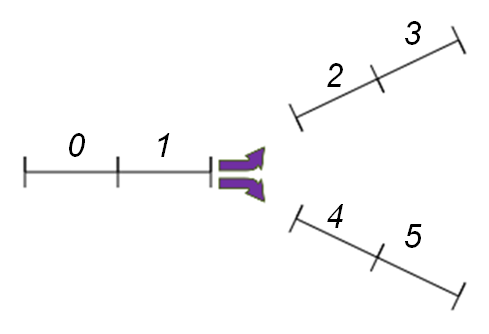
\includegraphics[width=10cm]{images/env_11_italic_no_perc}
	\label{fig:env_11}
	\caption{Numeracja odcinków środowiska}
\end{figure}Niech przykładowym wektorem stanu będzie:
\[\textbf{x}(t)=\xzero \addtag \]
Zawiera on w sobie informacje dotyczące liczby pojazdów na poszczególnych odcinkach w chwili t. Poniższy obraz przedstawia liczbę pojazdów na poszczególnych odcinkach dla stanu zadanego przez wektor $\textbf{x}(t)$.
\begin{figure}[H]
	\centering
	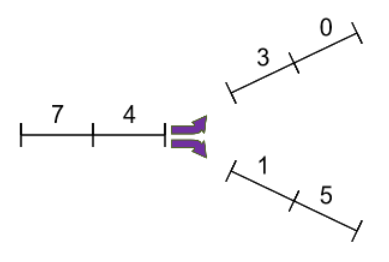
\includegraphics[width=10cm]{images/env_11_743015}
	\caption{Sieć dróg z liczbą pojazdów na poszczególnych odcinkach}
	\label{fig:3_single_road}
\end{figure}

\section{Rozwój wektora stanu sieci dróg w oparciu o CTM}
Przedstawiony zostanie rozwój stanu środowiska sieci dróg. Jako model ruchu wykorzystany zostanie model CTM opisany w sekcji \myref{sec:CTM}. W przypadku sieci dróg należy uwzględnić przypadek  gdy pojazdy mogą obrać różne kierunki ruchu (np. na skrzyżowaniu). W tym celu przedstawiona zostanie macierz prawdopodobieństwa. 
\subsection{Macierz prawdopodobieństwa} \label{sec:macierz_prawd}
\textbf{Macierz prawdopodobieństwa} \textbf{P} jest niezmienną w czasie rzadką macierzą. Wartości macierzy $P[j,i]$ określają jaka część pojazdów będących na odcinku $i$ ma zamiar przejazdu do odcinka $j$. Dla niemożliwych manewrów $[j,i]$ wartości macierzy $\textbf{P}$ są równe 0.
\subsubsection*{Przykład macierzy prawdopodobieństwa} \label{sec:p_example}
Rozważona zostanie poprzednia sieć dróg z dodatkowym założeniem, że 25 procent pojazdów ma zamiar dokonać manewru skrętu w lewo. Pozostałe 75 procent pojazdów z tego odcinka wybiera jazdę w prawo.

\begin{figure}[H]
	\centering
	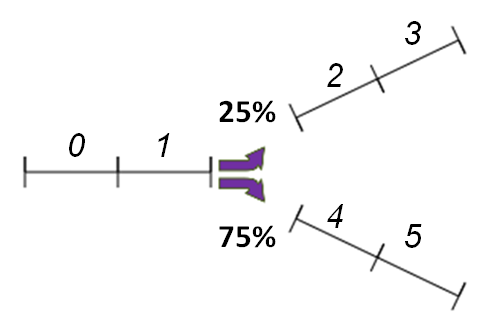
\includegraphics[width=10cm]{images/env_11_perc_italic}
	\label{fig:env_11}
	\caption{Sieć dróg z prawdopodobieństwami przejazdów}
\end{figure}

%\begin{tabular}{|  Sc | Sc|}
%	\hline
%	Numeracja odcinków & Liczba pojazdów \\
%	\hline
%	\cincludegraphics[width=8cm]{images/env_11_perc_italic} & 	\cincludegraphics[width=8cm]{images/env_11_743015_procenty} \\
%	\hline 
%\end{tabular} 
\noindent Wtedy macierz prawdopodobieństwa jest następująca:
\def \P {\begin{bmatrix}
		0 & 0 & 0 & 0 & 0 & 0 \\
		1 & 0 & 0 & 0 & 0 & 0 \\
		0 & 0.25 & 0 & 0 & 0 & 0 \\
		0 & 0 & 1 & 0 & 0 & 0 \\
		0 & 0.75 & 0 & 0 & 0 & 0 \\
		0 & 0 & 0 & 0 & 1 & 0 
\end{bmatrix}}
\[\textbf{P}=\P \addtag \label{eq:p_example} \]
Dodatnie wartości macierzy $P$ są następujące:
\begin{itemize}
	\item $P[1,0]=1$ - manewr jazdy prosto z odcinka 0 do 1
	\item $P[3,2]=1$ - manewr jazdy prosto z odcinka 2 do 3
	\item $P[5,4]=1$ - manewr jazdy prosto z odcinka 4 do 5
	\item $P[2,1]=0.25$ - manewr jazdy w lewo z odcinka 1 do 2
	\item $P[4,1]=0.75$ - manewr jazdy w prawo z odcinka 1 do 4
\end{itemize}
Wartości macierzy prawdopodobieństwa dla pierwszych trzech manewrów są równe 1, gdyż każdy pojazd na odcinku 0 ma zamiar przejechać na odcinek 1 (analogicznie z 2 na 3 oraz z 4 na 5). 25 procent pojazdów z odcinka 1 ma zamiar jazdy w lewo do odcinka 2. Z kolei pozostałe 75 procent chce obrać kierunek jazdy w prawo do odcinka 4. Kolumny odpowiadające odcinkom 3 i 5 mają wartości zerowe. Jest to uzasadnione tym, że pojazdy będące na tych odcinkach opuszczają układ.


\subsection{Macierz systemu}
%Przepływ pojazdów niezmiennie jest oparty o założenie, iż w trakcie trwania jednego interwału czasowego pojazdy pokonują 1 odcinek drogi. Nie pojawiają się nowe pojazdy w trakcie trwania symulacji, a ujścia ruchu znajdują się na końcu odcinków 3 i 5.
Przedstawiona w tej sekcji macierz systemu $\textbf{A}$ powinna uwzględnić przepływy pojazdów na skrzyżowaniach oraz model ruchu CTM. Opisy modelu ruchu CTM oraz oznaczeń użytych w poniższej definicji są zawarte w rozdziale \myref{sec:CTM}. Macierz systemu z następującymi wartościami gwarantuje przepływ zgodny z modelem ruchu CTM:
\begin{numcases}{A[j,i](t)=}
\frac{y_{ij}(t)}{x_i(t)} & dla $i \neq j$, $i \notin \Omega_{out}$ \label{eq:i_rozne_od_j} \\ 
\frac{x_{i}(t)-y_{i*}(t)}{x_i(t)} & dla $i=j$, $i \notin \Omega_{out}$ \label{eq:i_rowne_j} \\
0 & dla $i \in \Omega_{out} \label{eq:i_w_omega_out}$
\end{numcases}
Powyższy wzór wymaga dokładnego omówienia. Jest on zgodny z początkową definicją macierzy systemu \myref{sec:macierz_systemu_def}. Dla przypomnienia wartości macierzy systemu są określone jako część pojazdów będących na odcinku $i$ dokonujących manewru $[j,i]$. Zgodność wszystkich 3 przypadków jest omówiona poniżej:
\begin{itemize}
	\item \myref{eq:i_rozne_od_j} - Wartość $\frac{y_{ij}(t)}{x_i(t)}$ to stosunek pojazdów, które przejechały z odcinka $i$ do odcinka $j$ (tj. $y_{ij}(t)$) do całkowitej liczby pojazdów na odcinku $i$ (tj. $x_i(t)$).
	\item \myref{eq:i_rowne_j} - Wartość $y_{i*}(t)$ określa liczbę pojazdów, które opuściły odcinek $i$. Zatem licznik $x_{i}(t) - y_{i*}(t)$ to liczba pojazdów, które pozostały na odcinku $i$.
	\item \myref{eq:i_w_omega_out} - Odcinki bezpośrednio przed ujściem są oznaczane jako $\Omega_{out}$. Pojazdy będące na nich przejeżdżają do ujścia, zatem nie wjeżdżają do żadnego innego odcinka $j \in \Omega$,
\end{itemize}


\subsubsection*{Przykład} \label{sec:przyklad_CTM_skrz}
Rozważone zostanie środowisko (\ref{subsec:wektor_stanu_siec_przyklad}) z założeniem, że 75 procent pojazdów ma zamiar skręcić w prawo. Pozostałe 25 procent wybiera skręt w lewo. 
Środowisko przedstawiają poniższe obrazki oraz ustalenia.
\newline \newline
\begin{table}[H]
\begin{center}
\begin{tabular}{| Sc  | Sc |}
	\hline
	Numeracja odcinków   & Liczba pojazdów \\
	\hline
	\cincludegraphics[width=7cm]{images/env_11_perc_italic}  & \cincludegraphics[width=7cm]{images/env_11_743015_procenty} \\
	\hline\end{tabular}
\end{center}
\caption {Przykład środowiska z prawdopodobieństwami przepływu na skrzyżowaniu} \label{tab:cokolwiek}
\end{table}
\def \A{
\begin{bmatrix}
	0 & 0    & 0 & 0 & 0 & 0 \\
	1 & 0    & 0 & 0 & 0 & 0 \\
	0 & 0.25 & 0 & 0 & 0 & 0 \\
	0 & 0    & 1 & 0 & 0 & 0 \\
	0 & 0.75 & 0 & 0 & 0 & 0 \\
	0 & 0    & 0 & 0 & 1 & 0 
\end{bmatrix}
}
\def \Azero{
	\begin{bmatrix}
		\frac{4}{7} & 0    & 0 & 0 & 0 & 0 \\
		\frac{3}{7} & 0    & 0 & 0 & 0 & 0 \\
		0 & 0.25 & 0 & 0 & 0 & 0 \\
		0 & 0    & 1 & 0 & 0 & 0 \\
		0 & 0.75 & 0 & 0 & 0 & 0 \\
		0 & 0    & 0 & 0 & 1 & 0 
	\end{bmatrix}
} 
\begin{itemize}[nosep]
	\setlength\itemsep{0.5cm}
	\item Sposób przepływu przez skrzyżowanie z powyższego obrazka definiuje macierz prawdopodobieństwa $ \textbf{P} $ określoną w przykładzie \myref{eq:p_example}.
	\setlength\itemsep{0.5cm}
	\item Do sieci nie napływają żadne pojazdy, zatem wartości wektora źródła są równe 0 co jest zapisane jako $\textbf{u}(t)=\theta$ dla dowolnego $t$. 
	\setlength\itemsep{0.5cm}
	\item Liczba pojazdów będąca na odcinku jest ograniczona przez $N_j(t)=7$ dla dowolnego odcinka $i$ oraz chwili $t$.
	\setlength\itemsep{0.5cm}
	\item Maksymalny przepływ pojazdów w jednym interwale to $V_j(t)=4$	
\end{itemize} \vspace{0.4cm} \noindent
Wtedy następująca tabela przedstawia rozwój środowiska:
\def \xI{\begin{bmatrix}
		4 \\ 3 \\ 1 \\ 3 \\ 3 \\ 1
\end{bmatrix}}
\def \xII{\begin{bmatrix}
		0 \\ 4 \\ \frac{3}{4} \\ 1 \\ 2\frac{3}{4} \\ 3
\end{bmatrix}}
\def \xIII{\begin{bmatrix}
		0 \\ 0 \\ 0 \\ 6 \\ 0 \\ 2
\end{bmatrix}}
%\begin{flushleft}
\begin{table}
	\centerline{
\begin{tabular}{| c | c | Sc |}
	\hline
	t   & Równanie stanu & Podgląd środowiska \\
	\hline
	0 & 
	$ \textbf{x(0)} = \xzero$  & \cincludegraphics[width=7cm]{images/env_11_743015_procenty} \\
	\hline 
	1 & $\textbf{x(1)}=\textbf{A(0)x(0)}=\Azero \xzero = \xI$  & \cincludegraphics[width=7cm]{images/env_11_431331_procenty} \\
	\hline 
	2 & $\textbf{x(2)}=\textbf{A(1)x(1)}=\A \xI = \xII$  & \cincludegraphics[width=7cm]{images/env_11_04u1u3_procenty} \\
	\hline 
	3 &	$\textbf{x(3)}=\textbf{A(2)x(2)}=\A \xII = \xIII$ & \cincludegraphics[width=7cm]{images/env_11_000602_procenty} \\
	\hline 
\end{tabular}
}
\caption {Przepływ pojazdów} \label{tab:przeplyw}
\end{table}
%\end{flushleft}






\newpage
\section{Wprowadzenie sygnalizacji świetlnej} \label{sec:sygnalizacja}
Kolejnym etapem rozwoju modelu jest wprowadzenie sygnalizacji świetlnej. Warto zauważyć, że do tej pory rozważane układy były pozbawione jakiegokolwiek sterowania. Zostanie teraz zdefiniowana \textbf{macierz sygnalizacji świetlnej} $\textbf{S}(t)$. Jest ona zmienna w czasie, gdyż odpowiada za sterowanie sygnalizacją świetlną. Wartości macierzy sygnalizacji $S[j,i](t)$ określają, czy manewr $[j,i]$ jest wykonalny w chwili $t$.
\begin{numcases}{S[j,i](t)=}
1 & dla manewru zezwolonego przez zielone światło \label{eq:allowed_by_light} \\
1 & dla manewru nie wymagającego sygnalizacji świetlnej \label{eq:manewr_existing} \\
0 & dla manewru wstrzymanego przez czerwone światło \label{eq:stopped_by_light} \\
0 & dla niemożliwego manewru \label{eq:manewr_not_existing}
\end{numcases}
Sygnalizacja świetlna zwykle posiada pewną fazę, która określa dozwolone \myref{eq:allowed_by_light} oraz niedozwolone \myref{eq:stopped_by_light} manewry. Chociaż macierz sygnalizacji świetlnej jest zmienna w czasie to wartości macierzy $\textbf{S}$ dla manewrów niemożliwych \myref{eq:manewr_not_existing} oraz nie wymagających sygnalizacji świetlnej \myref{eq:manewr_existing} są niezmienne dla ustalonego środowiska.
\subsection*{Przykład macierzy sygnalizacji świetlnej} \label{subsec:macierz_sygnalizacji}
Rozważone będzie znane z poprzednich przykładów skrzyżowanie - tym razem mające sygnalizację świetlną z aktywną fazą zezwalającą na manewr [2,1]. Ta sama faza zabrania przejazdu z 1 odcinka do 4. \newline
\begin{figure}[H]
	\centering
	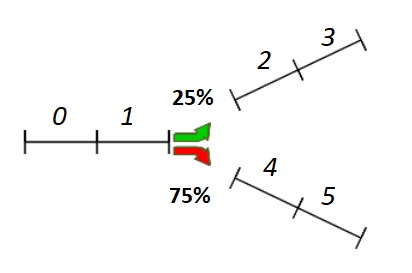
\includegraphics[width=10cm]{images/env_11_faza_0_procenty_italic}
	\label{fig:env_11}
	\caption{Przykład fazy sygnalizacji świetlnej}
\end{figure}

Poszczególne manewry są następujące:
\begin{itemize}
	\item \myref{eq:allowed_by_light} - Manewrem zezwolonym przez zielone światło  dla fazy $ 0 $ jest $ [2,1] $, czyli przejechanie na odcinek 2 z odcinka 1.
	\item \myref{eq:manewr_existing} - Prawidłowymi manewrami niewymagającymi sygnalizacji świetlnej są manewry $ [1,0] $, $ [3,2] $, $ [5,4] $.
	\item \myref{eq:stopped_by_light} - Dla fazy świetlnej $ 0 $ manewrem wstrzymanem przez czerwone światło jest $ [4,1] $.
	\item \myref{eq:manewr_not_existing} - Pozostałe manewry są niemożliwe. Przykładem jest $ [2,0] $, gdyż nie ma możliwości bezpośredniego przejazdu z odcinka $ 0 $ do $ 2 $.
\end{itemize}

Macierz sygnalizacji świetlnej dla tego przykładu jest następująca:
\def \S{\begin{bmatrix}
		0 & 0 & 0 & 0 & 0 & 0 \\
		1 & 0 & 0 & 0 & 0 & 0 \\
		0 & 0 & 0 & 0 & 0 & 0 \\
		0 & 0 & 1 & 0 & 0 & 0 \\
		0 & 0 & 0 & 0 & 0 & 0 \\
		0 & 0 & 0 & 0 & 1 & 0 \\
\end{bmatrix}}
\def \S_zero_one{
	\begin{bmatrix}
		0 & 0            & 0 & 0 & 0 & 0 \\
		1 & 0            & 0 & 0 & 0 & 0 \\
		0 & {\color[rgb]{0,.70,0} \textbf{1}}  & 0 & 0 & 0 & 0 \\
		0 & 0            & 1 & 0 & 0 & 0 & \\
		0 & {\color[rgb]{.70,0,0} \textbf{0}}  & 0 & 0 & 0 & 0 \\
		0 & 0            & 0 & 0 & 1 & 0 \\
	\end{bmatrix}
}
\[\textbf{S}= \S_zero_one \addtag \]
W dalszych rozważaniach {\color[rgb]{0,.70,0} \textbf{zielony kolor}} wartości macierzy sygnalizacji świetlnej odnosi się do zielonego światła dla manewru zadanego przez wiersz $j$ i kolumnę $i$. Analogicznie 
{\color[rgb]{.70,0,0} \textbf{czerwony kolor}} oznacza czerwone światło.
%\subsection{Rozwój wektora stanu sieci z sygnalizacją świetlną}
%Przepływ ruchu odbywa się zgodnie z opisanym w \myref{sec:CTM_sygnalizacja} przypadku modelu CTM z sygnalizacją świetlną. Jako parametry $s_{ij}(t)$ przypisane są wartości macierzy sygnalizacji świetlnej $\textbf{S(t)}$. Formuła macierzy systemu przedstawiona w 
%(\ref{eq:i_rozne_od_j}-\ref{eq:i_w_omega_out}) pozostaje niezmienna.
\subsection*{Przykład rozwoju wektora stanu} \label{sec:rozwoj_sieci_sygnalizcja_przypadek}
Przepływ ruchu odbywa się zgodnie z opisanym w \myref{sec:CTM_sygnalizacja} przypadku modelu CTM z sygnalizacją świetlną. Jako parametry $s_{ij}(t)$ przypisane są wartości macierzy sygnalizacji świetlnej $S(t)[j,i]$. Formuła macierzy systemu przedstawiona w 
(\ref{eq:i_rozne_od_j}-\ref{eq:i_w_omega_out}) pozostaje niezmienna. \newline
Niech będzie dany układ z przykładu \myref{subsec:macierz_sygnalizacji} z zielonym światłem dla lewoskrętu. W chwili $t=2$ zostanie zmieniona faza świetlna. Od tego momentu obydwa manewry na skrzyżowaniu są dozwolone.  
\def \xzero{\begin{bmatrix}
		9 \\ 4 \\ 3 \\ 0 \\ 1 \\ 5
\end{bmatrix}}
\def \xI{\begin{bmatrix}
		0 \\ 12 \\ 1 \\ 3 \\ 0 \\ 1
\end{bmatrix}}
\def \xII{\begin{bmatrix}
		0 \\ 9 \\ 3 \\ 1 \\ 0 \\ 0
\end{bmatrix}}
\def \xIII{\begin{bmatrix}
		0 \\ 0 \\ 2 \frac{1}{4} \\ 3 \\ 7 \frac{3}{4} \\ 0
\end{bmatrix}}

\def \AZero{
	\begin{bmatrix}
		0 & 0            & 0 & 0 & 0 & 0 \\
		1 & \frac{3}{4}  & 0 & 0 & 0 & 0 \\
		0 & \frac{1}{4}  & 0 & 0 & 0 & 0 \\
		0 & 0            & 1 & 0 & 0 & 0 & \\
		0 & 0            & 0 & 0 & 0 & 0 \\
		0 & 0            & 0 & 0 & 1 & 0 \\
	\end{bmatrix}	
}

\def \AI{
	\begin{bmatrix}
	0 & 0            & 0 & 0 & 0 & 0 \\
	1 & \frac{3}{4}  & 0 & 0 & 0 & 0 \\
	0 & \frac{1}{4}  & 0 & 0 & 0 & 0 \\
	0 & 0            & 1 & 0 & 0 & 0 & \\
	0 & 0            & 0 & 0 & 0 & 0 \\
	0 & 0            & 0 & 0 & 1 & 0 \\
\end{bmatrix}	
}
\def \AII{
	\begin{bmatrix}
	0 & 0            & 0 & 0 & 0 & 0 \\
	1 & 0            & 0 & 0 & 0 & 0 \\
	0 & \frac{1}{4}  & 0 & 0 & 0 & 0 \\
	0 & 0            & 1 & 0 & 0 & 0 & \\
	0 & \frac{3}{4}  & 0 & 0 & 0 & 0 \\
	0 & 0            & 0 & 0 & 1 & 0 \\
\end{bmatrix}
}

\begin{table}[H]
\centerline{
%\begin{center}
\begin{tabular}{| c | c | Sc |}
	\hline
	t   & Równanie stanu & Podgląd środowiska \\
	\hline
	0 &
	$ \textbf{x(0)} = \xzero$  & \cincludegraphics[width=7cm]{images/env_11_lights_0_943015_procenty} \\
	\hline 
	1 & $\textbf{x(1)}=\textbf{A(0)x(0)}=\AZero \xzero = \xI$  & \cincludegraphics[width=7cm]{images/env_11_lights_0_0121301_procenty} \\
	\hline 
	2 & $\textbf{x(2)}=\textbf{A(1)x(1)}=\AI \xI = \xII$  & \cincludegraphics[width=7cm]{images/env_11_lights_01_093100_procenty} \\
	\hline 
	3 &	$\textbf{x(3)}=\textbf{A(2)x(2)}=\AII \xII = \xIII$ & \cincludegraphics[width=7cm]{images/env_11_lights_koncowe_procenty} \\
	\hline 
\end{tabular}
} 
\caption{Przepływ pojazdów na skrzyżowaniu z sygnalizacją świetlną}
%\end{center}
\end{table}
\newpage
W chwili t=3 wartości stanu są niecałkowite, co nie jest sprzeczne z modelem makroskopowym. Rozwój wektora stanu został przedstawiony w poniższej tabeli.
%\color{blue!240}{cooo}
%{\color[rgb]{1,0,0} This text will appear red-colored}
Macierz sygnalizacji świetlnej dla $t=0,1$ jest następująca:
\[\textbf{S}(t)= \S_zero_one \addtag \]
Z kolei dla $t=2,3$:
\def \S_II_III{
	\begin{bmatrix}
		0 & 0            & 0 & 0 & 0 & 0 \\
		1 & 0            & 0 & 0 & 0 & 0 \\
		0 & {\color[rgb]{0,.70,0} \textbf{1}}  & 0 & 0 & 0 & 0 \\
		0 & 0            & 1 & 0 & 0 & 0 & \\
		0 & {\color[rgb]{0,.70,0} \textbf{1}}  & 0 & 0 & 0 & 0 \\
		0 & 0            & 0 & 0 & 1 & 0 \\
	\end{bmatrix}
}
\[\textbf{S}(t)=\S_II_III \addtag \]
\newpage
\section{Kolizyjność manewrów}
Manewrami kolizyjnymi nazywane są dwa manewry wjazdu na ten sam odcinek $j$. Przedstawiony model sieci dróg nie określa sposobu przepływu dla manewrów kolizyjnych w przypadku skrzyżowania bez sygnalizacji świetlnej. Wszystkie do tej pory skrzyżowania były jedynie rozwidleniem dróg lub posiadały sygnalizację świetlną. Poprawnie sformułowana faza świetlna nie posiada manewrów kolizyjnych. 


\subsection*{Przykład poprawnych faz}
Rozważone zostanie skrzyżowanie przedstawione poniżej. Każda droga wjazdowa posiada 3 manewry: skrętu w lewo, prawo i jazdy prosto.
\begin{figure}[H]
	\centering
	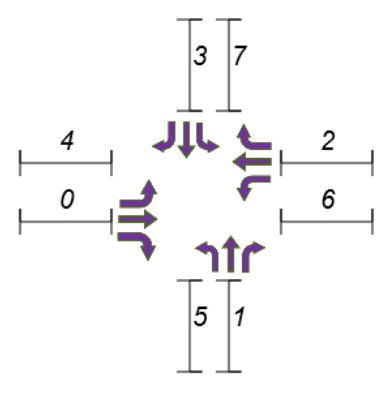
\includegraphics[width=10cm]{images/netx}
	\label{fig:cross_x}
	\caption{Rozważane skrzyżowanie}
\end{figure}
Przykłady poprawnych i niepoprawnych faz zostały zawarte w tabeli.
\begin{table}[H]
\begin{center}
\begin{tabular}{|  Sc | Sc|}
	\hline
	Poprawne fazy & Niepoprawne fazy \\
	\hline
	\cincludegraphics[height=6cm]{images/netx_faza_0} & 	\cincludegraphics[height=6cm]{images/netx_faza_0_n} \\
	\hline 
	\cincludegraphics[height=6cm]{images/netx_faza_1} & 	\cincludegraphics[height=6cm]{images/netx_faza_1_n} \\
	\hline 
	\cincludegraphics[height=6cm]{images/netx_faza_3} & 	\cincludegraphics[height=6cm]{images/netx_faza_2_n} \\
	\hline 
\end{tabular} 
\caption{Przykłady poprawnych i niepoprawnych faz sygnalizacji świetlnej}
\end{center}
\end{table}

\section{Wprowadzenie źródeł ruchu }
Wszystkie poprzednie przykłady układów ruchu drogowego szybko kończyły się stanem w którym nie było już żadnych pojazdów na drogach. W tej sekcji zostanie przedstawiony sposób napływania nowych pojazdów do układu. 
Wprowadzony zostanie wektor źródła $\textbf{u(}t\textbf{)}$. Jest on zmienny w czasie, a jego wartości określają ile pojazdów pojawia się w chwili $t+1$ na poszczególnych odcinkach układu. Równanie systemu uwzględniające źródła ruchu to:
\[\textbf{x(}t\textbf{)}=\textbf{A(}t\!-\!1\textbf{)}\textbf{x(}t\!-\!1\textbf{)} + \textbf{u(}t\!-\!1\textbf{)}. \label{eq:stan_u}   \addtag\]
\subsection*{Przykład}
Rozważony zostanie prosty przykład, który dla ułatwienia nie uwzględnia wcześniej wprowadzonych pojęć sygnalizacji świetlnej oraz zatoru. Przedstawione zostanie środowisko składające się z dwóch dróg, które nie są ze sobą w żaden sposób połączony.
\begin{figure}[H]
	\centering
	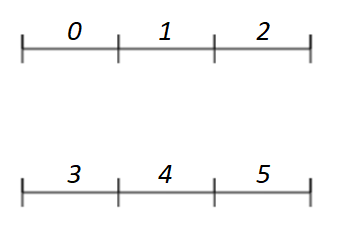
\includegraphics[width=8cm]{images/env_12_italic2}
	\label{fig:env_12}
	\caption{Numeracja odcinków środowiska}
\end{figure} \noindent
Pojazdy poruszają się z odcinków 0 (3) kończąc swój bieg po przejechaniu przez odcinki 5 (2) co przedstawia macierz systemu $\textbf{A}$:
\def \A{\begin{bmatrix}
0 & 0 & 0 & 0 & 0 & 0 \\
1 & 0 & 0 & 0 & 0 & 0 \\
0 & 1 & 0 & 0 & 0 & 0 \\
0 & 0 & 0 & 0 & 0 & 0 \\
0 & 0 & 0 & 1 & 0 & 0 \\
0 & 0 & 0 & 0 & 1 & 0
\end{bmatrix}}
\[\textbf{A}=\A \addtag \]
Dla ułatwienia powyższa macierz przedstawia środowisko bez zatorów.
Pragnąc by do odcinków $0$ i $3$  napływało odpowiednio po $4$, $8$, $20$ oraz $3$, $7$, $5$ pojazdów należy zdefiniować ciąg wektorów $\textbf{u}(t)$ w sposób przedstawiony w poniższej tabeli. \newline

\def \xzero{\begin{bmatrix}
		0 \\ 8 \\ 1 \\ 3 \\ 3 \\ 1
\end{bmatrix}}
\def \xI{\begin{bmatrix}
		4 \\ 0 \\ 8 \\ 3 \\ 3 \\ 3
\end{bmatrix}}
\def \xII{\begin{bmatrix}
		8 \\ 4 \\ 0 \\ 7 \\ 3 \\ 3
\end{bmatrix}}
\def \xIII{\begin{bmatrix}
		20 \\ 8 \\ 4 \\ 5 \\ 7 \\ 3
\end{bmatrix}}
\def \uZero{\begin{bmatrix}
		4 \\ 0 \\ 0 \\ 3 \\ 0 \\ 0
\end{bmatrix}}
\def \uI{\begin{bmatrix}
		8 \\ 0 \\ 0 \\ 7 \\ 0 \\ 0
\end{bmatrix}}
\def \uII{\begin{bmatrix}
		20 \\ 0 \\ 0 \\ 5 \\ 0 \\ 0
\end{bmatrix}}
\begin{table}[H]
\centerline{
\begin{tabular}{| Sc | Sc | Sc | Sc |}
	\hline
	t   & Równanie stanu & Podgląd środowiska & $ \textbf{u}(t) $ \\
	\hline
	0 & 
	$ \textbf{x}(0) = \xzero$  & \cincludegraphics[width=5cm]{images/env_12_t0} & $\uZero$ \strut\\
	\hline 
	1 & $\textbf{x}(1)=\textbf{Ax}(0)+\textbf{u}(0)=\A \xzero + \uZero = \xI$ \strut  & \cincludegraphics[width=5cm]{images/env_12_t1} & $\uI $ \\
	\hline 
	2 & $\textbf{x}(2)=\textbf{Ax}(1)+\textbf{u}(1)=\A \xI + \uI = \xII$  & \cincludegraphics[width=5cm]{images/env_12_t2} & $\uII $ \\
	\hline 
	3 & \newline	\newline \newline $\textbf{x}(3)= \textbf{Ax}(2)+\textbf{u}(2)=\A \xII + \uII = \xIII$ & \cincludegraphics[width=5cm]{images/env_12_t3} & \\
	\hline 
\end{tabular}
}
\caption{Rozwój środowiska z uwzględnieniem źródeł ruchu}
\end{table}
 
\chapter {Środowiska symulacyjne i ich nauka}\label{chapter:envs}
W tym rozdziale przedstawione zostaną środowiska symulacyjne. Głównym ich elementem jest sieć dróg. Podstawowe informacje na temat działania modelu sieci dróg i ruchu obowiązującego na nich zostały przedstawione w rozdziale \ref{chapter:model_sieci_drog}. Każde środowisko posiada dokładną specyfikacje możliwych faz świetlnych, przestrzeni decyzyjnej i konsekwencji każdej z akcji. Na początku zostaną przedstawione ustalenia wspólne dla wszystkich środowisk uczenia.

\subsection*{Cel uczenia}
Celem uczenia jest uzyskanie jak największej liczby pojazdów, które opuściły układ.

\subsection*{Sygnał nagrody}
Do każdego ze skrzyżowań jest przyporządkowany agent, który ma za zadanie podejmować akcje prowadzące do ustalonego celu. Nagroda jest liczbą pojazdów, które właśnie przejechały przez skrzyżowanie przypisane do agenta.
\subsection*{Współczynnik dyskontujący}
Współczynnik dyskontujący został we wszystkich środowiskach ustalony jako $\gamma=0,9$.
\subsection*{Szybkość uczenia}
Parametr szybkości uczenia algorytmu Q-learning został ustalony na wartość $\alpha=1$. Jest to optymalna wartość tego parametru dla środowisk deterministycznych \cite{reinforcementBook}.
\subsection*{Podział danych na trening i walidację}
Ustalone zostaje, że 80 procent danych wygenerowanych podczas epizodów treningowych zostaje przeznaczonych do zbioru treningowego, a pozostałe 20 procent tworzy zbiór walidacyjny. 
\section{Środowisko 1}
%(11 na froncie)
Elementy sieci dróg pierwszego środowiska były niejednokrotnie przedstawiane w rozdziale \ref{chapter:model_sieci_drog}, jednak dopiero teraz nastąpi przedstawienie pierwszego pełnego środowiska symulacyjnego. Na model sieci składają się 3 drogi - każda ma po 2 odcinki. Jest jedno skrzyżowanie na którym 75 procent pojazdów skręca w prawo, a pozostałe obierają kierunek w lewo.
\begin{figure}[H]
	\centering
	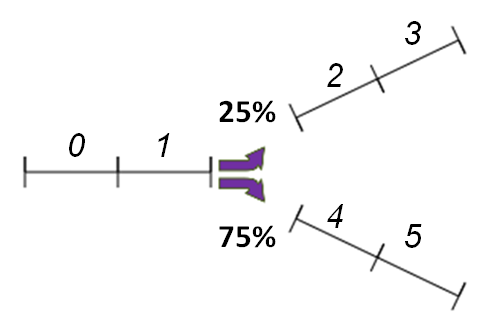
\includegraphics[width=10cm]{images/env_11_perc_italic}
	\label{fig:env_11}
	\caption{Środowisko 1}
\end{figure}

\subsection{Sygnalizacje świetlne}	
\begin{figure}[H]
	\centering
	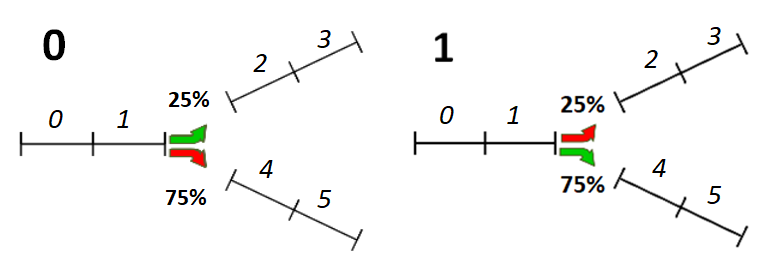
\includegraphics[width=17cm]{images/env_11_fazy_procenty_no_yellow_italic2}
	\label{fig:env_11_fazy}
	\caption{Środowisko 1 - fazy świateł}
\end{figure}\noindent
Skrzyżowanie posiada 2 fazy świetlne przedstawione powyżej. Faza 0 umożliwia skręt w lewo (manewr [1,2]) z kolei faza 1 umożliwia skręt w prawo (manewr [1,4]). Środowisko nie posiada żółtych świateł.

\subsection{Przestrzeń decyzyjna}
Agent ma dwie możliwe akcje do podjęcia - 0 oraz 1. Obydwie powodują natychmiastową aktywacje odpowiadającej im fazy świetlnej.

\subsection{Model ruchu}
Jako model ruchu zostanie wykorzystany przepływ CTM z następującymi parametrami:
\begin{itemize}
	\item Liczba pojazdów na odcinku jest nieograniczona tj. $N_j(t)=\infty$ dla dowolnych $j,t$.
	\item Maksymalna liczba pojazdów, które mogą napłynąć do odcinka to $V_j(t)=10$ dla dowolnego $j,t$.
	\item Ze źródła ruchu napływa w każdym interwale po 7 pojazdów do odcinka 0.
	\item Macierze prawdopodobieństwa $\textbf{P}$ i sygnalizacji $\textbf{S}$ są analogiczne do tych przedstawionych w \myref{sec:p_example} i \myref{subsec:macierz_sygnalizacji}.
\end{itemize}

\subsection{Uczenie}
\subsubsection*{Pożądane zachowanie}
Zazwyczaj więcej pojazdów ma szansę przejechać przez skrzyżowanie w trakcie fazy 1. Wyjątkiem są dwie sytuacje. Jeśli nie ma pojazdów przed rozwidleniem dróg - faza jest obojętna, gdyż i tak żaden pojazd nie przejedzie przez skrzyżowanie. Z kolei gdy pojazdów na odcinku przed skrzyżowaniem jest co najmniej 40, to zarówno faza 0 jak i 1 powodują przejazd 10 pojazdów. W pozostałych przypadkach to faza 1 jest bardziej opłacalna, gdyż pozwala na przejazd większej liczby pojazdów.
\subsubsection*{Sygnał wejściowy}
Sygnał wejściowy $\textbf{x}$ to liczby pojazdów na odcinkach przed skrzyżowaniem.
\subsubsection*{Przykład sygnału wejściowego}
Sygnał wejściowy $ \textbf{x}=[4,7] $ zawiera w sobie informację, iż na odcinku zerowym są 4 pojazdy oraz na pierwszym - jest ich 7. 
\subsubsection*{Sposób uczenia}
Zastosowana została metoda uczenia przedstawiona w \myref{learning:DQN_single_agent}. Szczegóły dotyczące sposobu uczenia są następujące:
\begin{itemize}
	\item $\epsilon = 1$ - akcje są wybierane w pełni losowy sposób podczas epizodów treningowych.
	\item Generowanych jest jednorazowo 50 epizodów treningowych. Każdy ma 90 interwałów czasowych.
	\item Warunkiem stopu jest 60 sekund działania algorytmu.
	\item Za uczenie odpowiada sieć neuronowa biblioteki Keras. Jej struktura jest następująca:  
	\begin{itemize}
		\item Posiada 2 ukryte warstwy, każda z 5 neuronami.
		\item Funkcja aktywacji zadana jest wzorem $f(x)=max({0,x})$, znana powszechnie jako ReLu (ang. \emph{Rectified Linear Unit})
		\item Optymalizacja jest przeprowadzana przez metodę Adam \cite{adam} z parametrem $learning\_rate = 0,01$
	\end{itemize}
\end{itemize}

%Posiada ona 2 ukryte warstwy, każda z 5 neuronami. Funkcją aktywacji zadana jest wzorem $f(x)=max({0,x})$, znana powszechnie jako ReLu (ang. \emph{Rectified Linear Unit}). Optymalizacja jest przeprowadzana przez metodę Adam z funkcją straty błędu średniokwadratowego i parametrem $learning\_rate = 0,01$.


\subsubsection{Wyniki uczenia}
Algorytm osiąga pożądane zachowanie. Na samym początku epizodu, gdy nie ma żadnych pojazdów przed skrzyżowaniem agent podejmuje różne akcje. W chwili gdy pojawiają się pojazdy zawsze wybrana jest akcja 1. Nie tworzą się zatory i wszystkie pojazdy opuszczają skrzyżowanie (oczywiście z wyjątkiem części tych, które pojawiły się w trzech ostatnich interwałach czasowych).
\section{Środowisko 2}
%(14 na froncie)
Na model sieci składają się 3 drogi - każda ma po 2 odcinki. Istnieje jedno skrzyżowanie z dwiema drogami wlotowymi i jedną wylotową.
	\begin{figure}[H]
	\centering
	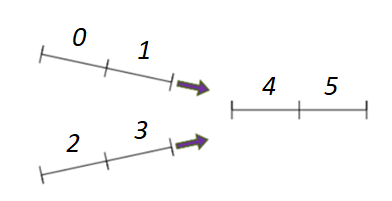
\includegraphics[width=10cm]{images/env_14_italic2}
	\label{fig:env_14}
	\caption{Środowisko 2}
\end{figure}

\subsection{Sygnalizacje świetlne}	
\begin{figure}[H]
	\centering
	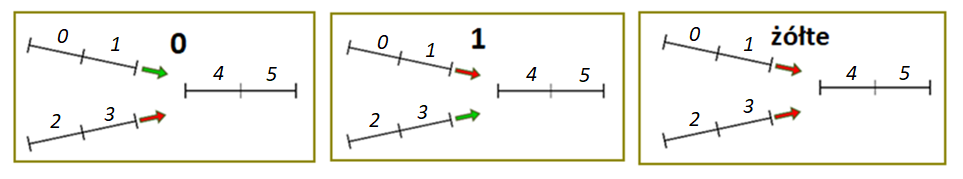
\includegraphics[width=17cm]{images/env_14_fazy_italic3}
	\label{fig:env_14_fazy}
	\caption{Środowisko 2 - fazy świateł}
\end{figure}\noindent
Skrzyżowanie posiada 3 fazy świetlne przedstawione powyżej. Faza 0 umożliwia przejazd przez skrzyżowanie z górnej drogi (manewr [1,4]) z kolei faza 1 umożliwia wjazd z drogi dolnej (manewr [3,4]). Faza `żółte` blokuje przejazd przez skrzyżowanie.

\subsection{Przestrzeń decyzyjna}
Przestrzeń decyzyjną oraz konsekwencje akcji podjętych przez agenta przedstawia poniższa tabela:
\begin{figure}[H]
	\centering
	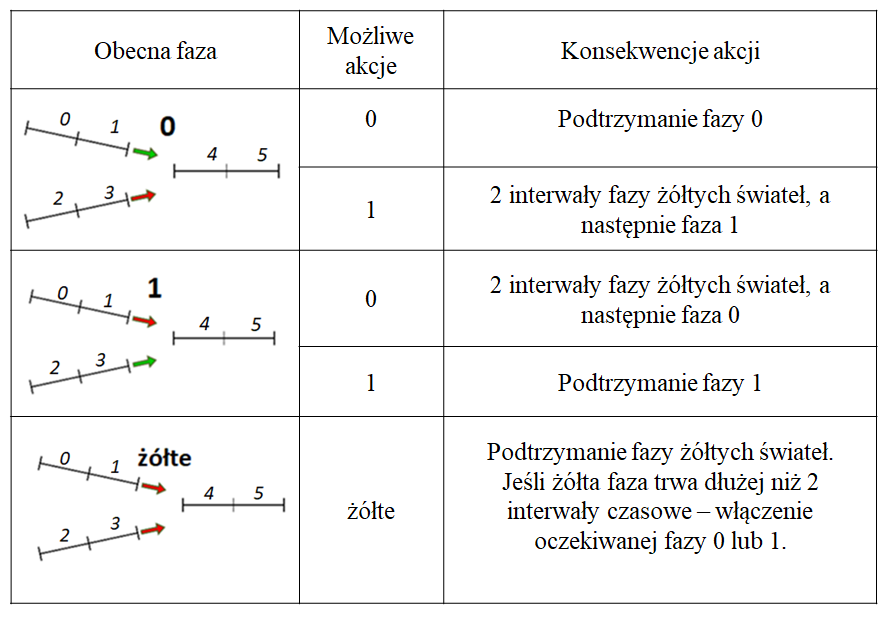
\includegraphics[width=16cm]{images/env_14_akcje_italic}
	\label{fig:env_14_akcje}
	\caption{Przestrzeń decyzyjna środowiska}
\end{figure} \noindent

\subsection{Model ruchu}
Jako model ruchu zostanie wykorzystany przepływ CTM z następującymi parametrami:
\begin{itemize}
	\item Liczba pojazdów na odcinku jest nieograniczona tj. $N_j(t)=\infty$ dla dowolnych odcinków $j$ i czasu $t$.
	\item Maksymalna liczba pojazdów, które mogą napłynąć do odcinka to $V_j(t)=10$ dla dowolnego $j,t$.
\end{itemize}

\subsection{Uczenie}
\subsubsection{Ogólny zarys}
Początkowo do każdej z dróg wjeżdżają po 2 pojazdy w jednym interwale czasowym. Przeprowadzona zostaje jedna iteracja nauki \myref{learning:DQN_single_agent}, po której następuje epizod testowy. Agent ma za zadanie wykonywać w trakcie niego akcje, które pozwolą na opuszczenie skrzyżowania przez co najmniej 98 procent pojazdów. W przypadku spełnienia tego warunku następuje zwiększenie liczby wjeżdżających do układu pojazdów. Następnie przeprowadzana jest kolejna iteracja uczenia \myref{learning:DQN_single_agent}. Ten proces jest powtarzany, aż do momentu gdy w trakcie 10 kolejnych epizodów testowych nie uzyskany zostanie warunek 98 procent pojazdów opuszczających skrzyżowanie. 
\subsubsection{Spodziewany wynik}
Koniec nauki spodziewany jest na chwilę, gdy na każdą z dróg będzie wjeżdżało około 5 pojazdów (w sumie 10 pojazdów do układu). Zgodnie z opisem modelu ruchu - maksymalnie 10 pojazdów może przejechać w jednej chwili przez skrzyżowanie, zatem muszą się tworzyć zatory przy większej liczbie pojazdów.
\subsubsection{Pożądane zachowanie agenta}
Pożądane zachowanie agenta w tym przypadku nie jest jednoznaczne do określenia. Z pewnością jeśli na drodze na której jest zielone światło jest co najmniej 10 pojazdów, to warto podtrzymać fazę świetlną. Zmiana sygnalizacji powoduje 2 interwały karencji, podczas których żaden pojazd nie przejedzie i może to być czynnikiem decydującym o pozostaniu przy obecnej fazie. Jaka powinna być akcja w przypadku gdy zielone światło jest dla drogi z mniejszą niż 10 liczbą pojazdów? Wtedy agent powinien odnaleźć złoty środek i jeśli na drugiej drodze jest dużo pojazdów - może zmienić światło.

\subsubsection*{Sygnał wejściowy}
Sygnał wejściowy posiada 4 wartości. Pierwsze dwie z nich to liczba pojazdów przed skrzyżowaniem. Kolejne określają aktualną fazę świetlną.
\subsubsection*{Przykłady sygnałów wejściowych}
\begin{itemize}
	\item Sygnał wejściowy $ \textbf{x}=[8,2,0,1] $ zawiera w sobie informację, iż na odcinku pierwszym jest 8 pojazdów oraz na trzecim - jest ich 2. Aktywna jest faza 1.
		\item Sygnał wejściowy $ \textbf{x}=[7,5,1,0] $ zawiera w sobie informację, iż na odcinku pierwszym jest 7 pojazdów oraz na trzecim - jest ich 5. Aktywna jest faza 0.
\end{itemize}
\subsubsection{Sposób uczenia}
Następujące stałe oraz ustalenia określają szczegóły uczenia:
\begin{itemize}
	\item Parametr $\epsilon$ jest początkowo równy 1 (w pełni losowe epizody). Z każdą iteracją jest zmniejszany o 0,01 aż do wartości $\epsilon=0,2$.
	\item Generowanych jest jednorazowo 10 epizodów treningowych. Każdy z nich trwa 1000 interwałów czasowych.
	\item Za uczenie odpowiada sieć neuronowa biblioteki Keras. Jej struktura jest następująca:  
	\begin{itemize}
		\item Posiada 3 ukryte warstwy (10,14,10 neuronów).
		\item Funkcja aktywacji zadana jest wzorem $f(x)=max({0,x})$, znana powszechnie jako ReLu (ang. \emph{Rectified Linear Unit})
		\item Optymalizacja jest przeprowadzana przez metodę Adam \cite{adam} z parametrem $learning\_rate = 0,01$
	\end{itemize}
\end{itemize}

\subsubsection*{Wyniki uczenia}
Algorytm szybko uzyskuje kolejne warunki 98 procent pojazdów przejeżdżających przez skrzyżowanie. Dopiero przy 4,97 wjeżdżających pojazdach na drogę (9,94 w sumie do układu) tworzą się zatory powodujące warunek stopu.
Najlepszy wynik to średnio 9,48 pojazdów przejeżdżających w jednej chwili przez skrzyżowanie. Jest to dobry wynik zważając na to, iż potencjalnie najwyższy możliwy wynik do osiągnięcia jest w granicy 9,94. Z 9940 pojazdów jedynie 450 nie opuściło skrzyżowania. Zatem przy niemalże 5 pojazdach napływających do układu powstają korki, co jest naturalnym zjawiskiem - wynikającym z ograniczeń ruchu, a nie nieoptymalnej sygnalizacji świetlnej.

\section{Środowisko 3}
%(16 na froncie)
\begin{figure}[H]
	\centering
	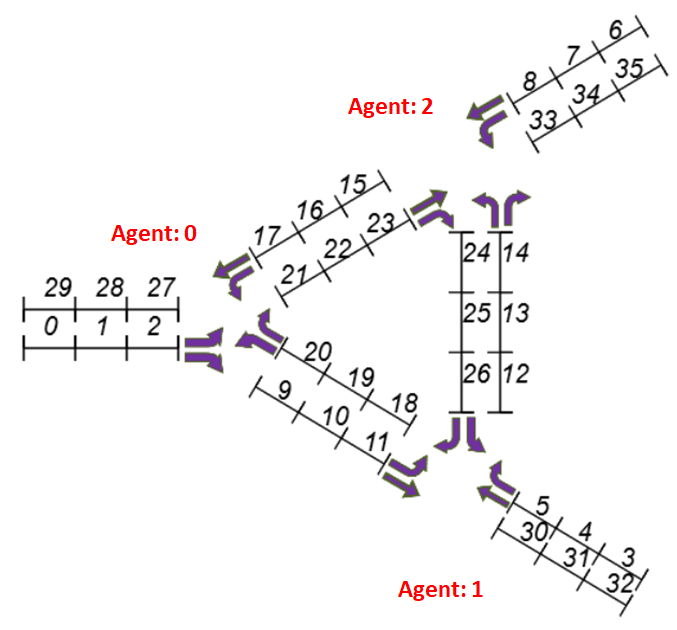
\includegraphics[width=12cm]{images/env_4_agenci_italic_no_perc}
	\label{fig:env_4_agenci}
	\caption{Środowisko 3}
\end{figure}


Środowisko posiada 12 jednokierunkowych dróg. Każda droga ma 3 odcinki co daje w sumie 36 odcinków (są numerowane od 0 co widać na rysunku \ref{fig:env_4_agenci}).
W sieci dróg znajdują się 3 skrzyżowania. Do każdego z nich jest przypisany agent, który odpowiada za sterowanie sygnalizacją świetlną.
\subsection{Sygnalizacje świetlne}
Każde skrzyżowanie posiada 4 fazy świetlne przedstawione poniżej. Fazy 0,1 i 2 są fazami, które posiadają pewne zielone światła. Zmiana pomiędzy tymi fazami nie jest natychmiastowa i następuje dopiero po 2 interwałach fazy żółtych świateł.
\begin{figure}[H]
	\centering
	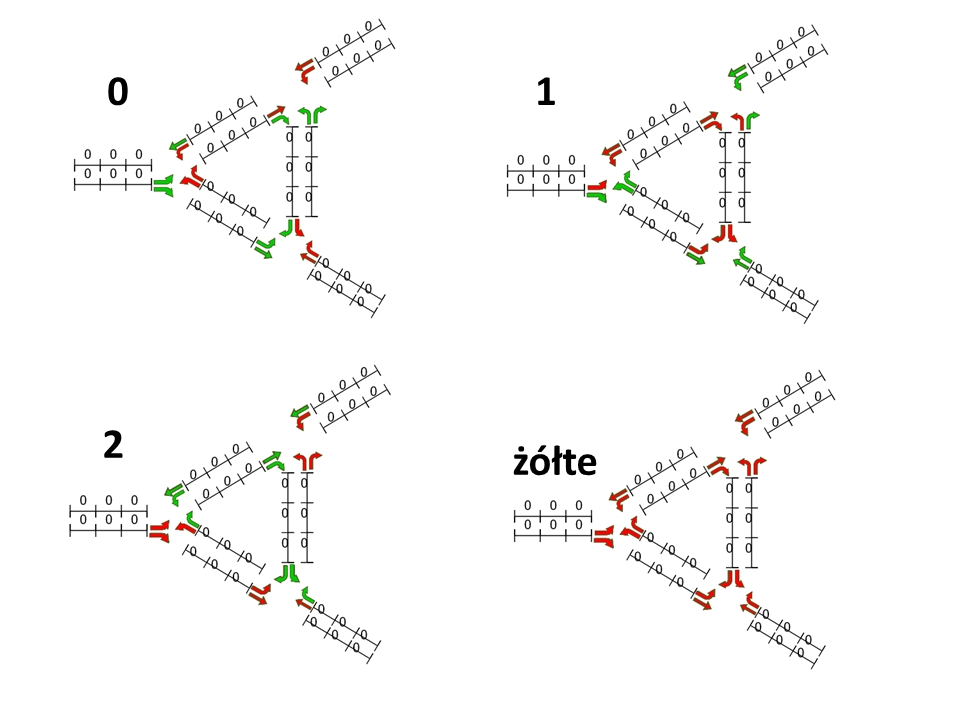
\includegraphics[width=14cm]{env_4_fazy}
	\label{fig:env_4_fazy}
	\caption{Środowisko 3 - fazy świateł}
\end{figure}
\subsection{Przestrzeń decyzyjna} \label{subsec_pn_dec}
Przedstawiona zostanie przestrzeń decyzyjna jedynie dla agenta 0, jednak dla pozostałych dwóch agentów przestrzenie decyzyjne są analogiczne. Schemat zmiany faz świetlnych jest identyczny, jedynie manewry faz są inne.
\begin{figure}[H]
	\centering
	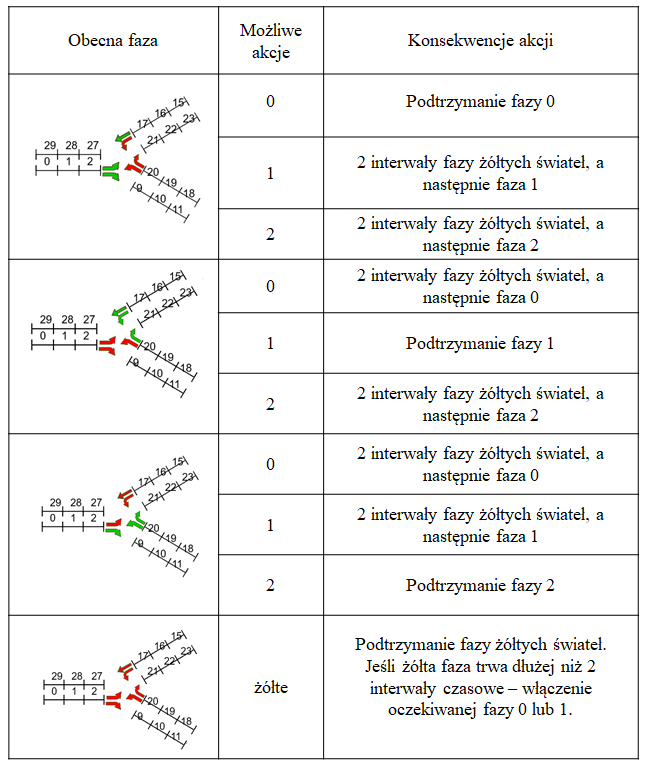
\includegraphics[width=14cm]{images/env_14_akcje_agent0_tabela}
	\label{fig:env_4_akcje_agent_0}
	\caption{Środowisko 3 - fazy świateł}
\end{figure}
\subsection{Model ruchu}
Jako model ruchu zostanie wykorzystany przepływ CTM z następującymi parametrami:
\begin{itemize}
	\item Liczba pojazdów na odcinku jest nieograniczona tj. $N_j(t)=\infty$ dla dowolnego odcinka $j$ i czasu $t$.
	\item Maksymalna liczba pojazdów, które mogą napłynąć do odcinka to $V_j(t)=10$ dla dowolnego $j,t$.
	\item Macierze sygnalizacji świetlnej $\textbf{S}$ są zgodne z fazami przedstawionymi w tabeli \myref{fig:env_4_akcje_agent_0}
	\item Macierze prawdopodobieństwa przejazdów $\textbf{P}$ są zgodne z przepływami przedstawionymi poniżej \myref{fig:srodowisko_3_przeplywy}. Jeśli na skrzyżowaniu jest dostępny manewr wyjazdu z sieci dróg, to 70 procent pojazdów obiera go. Jeśli nie ma takiego manewru, to 70 procent pojazdów skręca w prawo. Jedynie manewr $[15,8]$ jazdy prosto obiera 70 procent pojazdów. Reszta manewrów jest wybierana przez pozostałe 30 procent pojazdów. 
\end{itemize}
\begin{figure}[H]
	\centering
	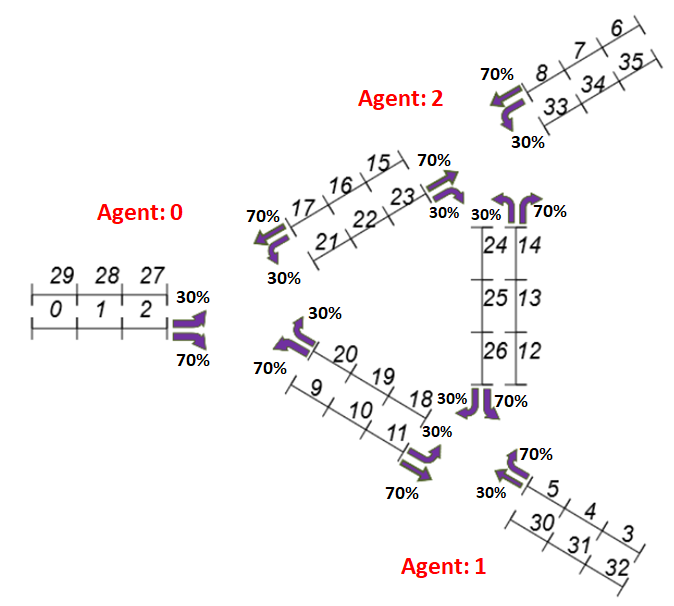
\includegraphics[width=14cm]{images/srodowisko_3_przeplywy_italic}
	\label{fig:srodowisko_3_przeplywy}
	\caption{Środowisko 3 - przepływy na skrzyżowaniach}
\end{figure}
\subsection{Uczenie}
\subsubsection{Ogólny zarys}
Początkowo do każdej z dróg wjeżdża po jednym pojeździe. Na koniec każdej iteracji nauki \myref{learning:DQN_single_agent} przeprowadzany jest epizod testowy. Agent ma za zadanie wybierać akcje, które pozwolą na opuszczenie sieci dróg przez co najmniej 93 procent pojazdów. Jeśli ten warunek zostanie spełniony następuje zwiększenie liczby wjeżdżających pojazdów o 20 procent dotychczasowej wartości. W przypadku gdy ten warunek nie zostanie spełniony w trakcie 15 kolejnych epizodów testowych następuje koniec nauki. 


\subsubsection*{Spodziewany wynik}
Moment stopu spodziewany jest na chwilę, gdy na każdą z dróg będzie wjeżdżało niecałe 10 pojazdów. Zgodnie z opisem modelu ruchu - maksymalnie 10 pojazdów może wjechać w jednej chwili na dany odcinek, zatem muszą się tworzyć zatory przy większej liczby pojazdów.


\subsubsection*{Sygnał wejściowy}
Sieć neuronowa przypisana do każdego z agentów przyjmuje jako sygnał wejściowy 6 elementową tablicę. Pierwsze 3 elementy to liczby pojazdów na odcinkach będących przed skrzyżowaniem przypisanym do agenta. Pozostałe 3 elementy mają wartości z zakresu $\{0,1\}$. Określają one aktualną fazę świetlną. 
\subsubsection*{Przykład sygnału wejściowego}
Sygnał wejściowy $\textbf{x}=[5,17,2,0,0,1]$ przedstawia informację, iż przed skrzyżowaniem są kolejki odpowiednio 5,17 i 2 pojazdów. Ostatnie 3 elementy oznaczają, że aktualna faza świetlna to 2.

\subsubsection*{Sposób uczenia}
Następujące stałe oraz ustalenia określają szczegóły uczenia:
\begin{itemize}
	\item Parametr zachłanności $\epsilon$ jest początkowo równy 1 (w pełni losowe epizody). Z każdą iteracją jest zmniejszany o 0,04 aż do wartości $\epsilon=0,2$.
	\item Generowanych jest jednorazowo 20 epizodów treningowych. Każdy z nich trwa 300 interwałów czasowych.
	\item Epizod testowy trwa 1000 interwałów czasowych.
	\item Za uczenie odpowiada sieć neuronowa biblioteki Keras. Jej struktura jest następująca:  
	\begin{itemize}
		\item Posiada 3 ukryte warstwy (10,14,10 neuronów).
		\item Funkcja aktywacji zadana jest wzorem $f(x)=max({0,x})$, znana powszechnie jako ReLu (ang. \emph{Rectified Linear Unit})
		\item Optymalizacja jest przeprowadzana przez metodę Adam \cite{adam} z parametrem $learning\_rate = 0,01$
	\end{itemize}
\end{itemize}
\subsubsection{Wyniki uczenia}
Moment stopu jest osiągnięty przy 8.9 pojazdów napływających do sieci ruchu. Najwyższy osiągnięty wynik to $24030$ pojazdów opuszczających układ. Jest to 90 procent napływających do środowiska pojazdów. Żadna z akcji nie jest zaniechana - agenci co najmniej kilkadziesiąt razy podejmują każdą z dostępnych akcji w zachłannym epizodzie.

\section{Środowisko 4 - kampus B Politechniki Łódzkiej}
\begin{figure}[H]
	\centering
	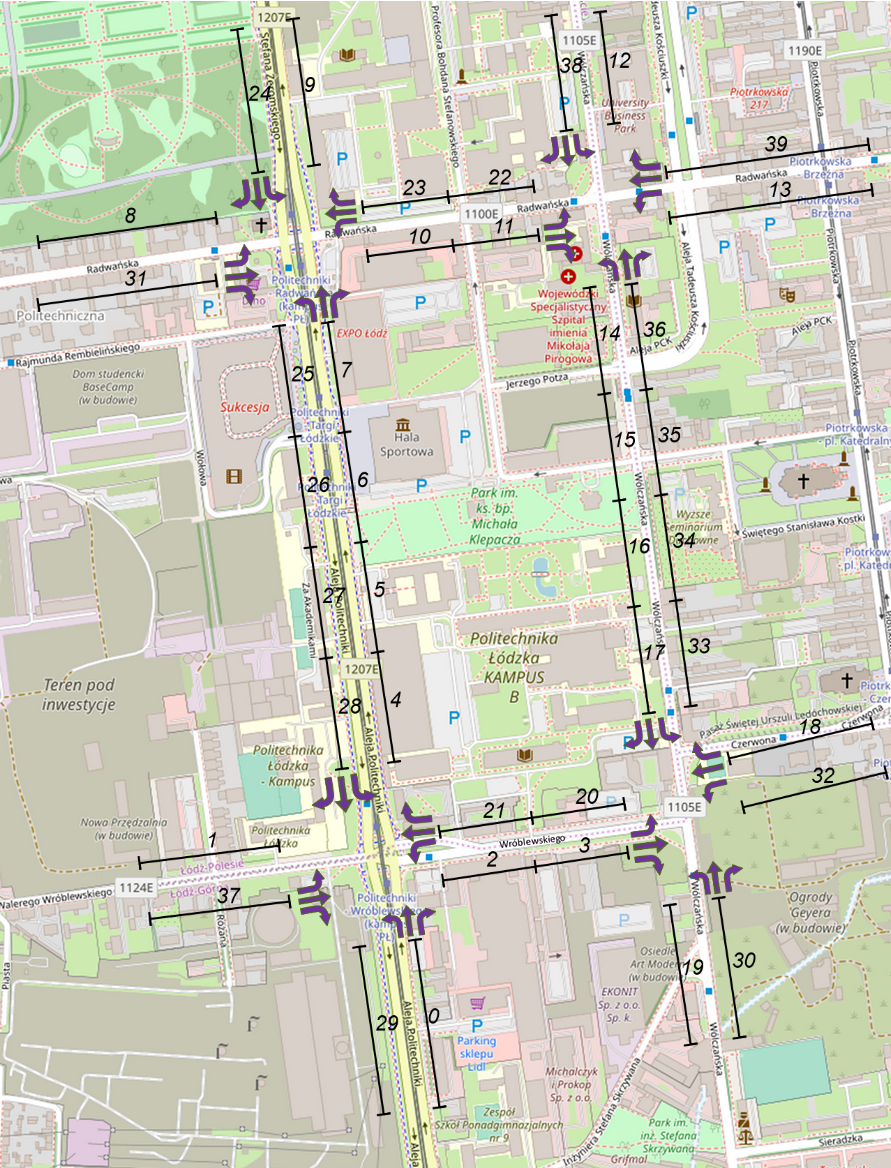
\includegraphics[width=12cm]{images/env_poli_italic2}
	\label{fig:env_poli}
	\centering
	\caption{Środowisko 5 - Skrzyżowania wokół kampusu B Politechniki Łódzkiej. Mapy Open Street Map \cite{OpenStreetMap}}
\end{figure}
Struktura środowiska bazuje na rzeczywistej sieci dróg znajdującej się w Łodzi. Sieć wyznaczają ulice Wróblewskiego, Wólczańska, Radwańska i aleja Politechniki Łódzkiej. Środowisko posiada 40 odcinków w tym 8 odcinków źródłowych (0,18,24,30,31,37,38,39) i 8 bezpośrednio przed ujściem ruchu (1,8,9,12,13,19,29,32). Drogi krzyżują się w 4 miejscach. Na dowolnym skrzyżowaniu kierowcy mogą wykonać manewry skrętu w lewo, w prawo oraz jazdy prosto. 


\subsection{Sygnalizacje świetlne}
Każde skrzyżowanie posiada 5 faz świetlnych. Fazy 0,1,2 i 3 są fazami, które posiadają pewne zielone światła. Zmiana pomiędzy tymi fazami nie jest natychmiastowa i następuje dopiero po 2 interwałach fazy żółtych świateł. W rzeczywistym skrzyżowaniu nie ma miejsca do wyminięcia się dla pojazdów skręcających w lewo z ulic Wróblewskiego i Czerwonej. Z tego względu skrzyżowanie ulic Wróblewskiego, Wólczańskiej i Czerwonej posiada inne od pozostałych trzech skrzyżowań fazy świetlne. Wynika to z kolizyjności lewoskrętów z ulic Wróblewskiego i Czerwonej. Poniższa tabela przedstawia możliwe fazy świetlne.
\begin{table}[H]
	\begin{center}
\begin{tabular}{| Sc  | Sc | Sc|}
	\hline
	Faza   & \specialcell{Wólczańska/\\Wróblewskiego/\\Czerwona} & Pozostałe 3 skrzyżowania \\
	\hline
	0  & 
	\cincludegraphics[height=4cm]{images/env_poli_faza_0_wol} & 	\cincludegraphics[height=4cm]{images/env_poli_faza_0_pozostale} \\
	\hline 
	1  & 
	\cincludegraphics[height=4cm]{images/env_poli_faza_1_wol} & 	\cincludegraphics[height=4cm]{images/env_poli_faza_1_pozostale} \\
	\hline 
	2  & 
	\cincludegraphics[height=4cm]{images/env_poli_faza_2_wol} & 	\cincludegraphics[height=4cm]{images/env_poli_faza_2_pozostale} \\
	\hline 
	3  & 
	\cincludegraphics[height=4cm]{images/env_poli_faza_3_wol} & 	\cincludegraphics[height=4cm]{images/env_poli_faza_3_pozostale} \\
	\hline 
	Żółte  & 
	\cincludegraphics[height=4cm]{images/env_poli_faza_zolte_wol} & 	\cincludegraphics[height=4cm]{images/env_poli_faza_zolte_pozostale} \\
	\hline 
\end{tabular} \label{fig:env_poli_akcje_agent_0}
\end{center}
\caption{Fazy świetlne środowiska}
\end{table}



\subsection{Przestrzeń decyzyjna}
Analogiczna do poprzednich przestrzeni decyzyjnych z fazą żółtych świateł - przykładowo \myref{subsec_pn_dec}.
\subsection{Model ruchu}
Jako model ruchu zostanie wykorzystany przepływ CTM z następującymi parametrami:
\begin{itemize}
	\item Liczba pojazdów na odcinku jest nieograniczona tj. $N_j(t)=\infty$ dla dowolnego odcinka $j$ i czasu $t$.
	\item Maksymalna liczba pojazdów, które mogą napłynąć do odcinka to $V_j(t)=10$ dla dowolnego $j,t$.
	\item Macierze sygnalizacji świetlnej $\textbf{S}$ są zgodne z fazami przedstawionymi w powyższej tabeli z sekcji \myref{fig:env_poli_akcje_agent_0}
	\item Macierze prawdopodobieństwa przejazdów $\textbf{P}$ uwzględniają następujące proporcje obierania kierunków. Jazdę prosto obiera połowa pojazdów. Manewr skrętu w prawo dokonuje 30 procent pojazdów, a w lewo ma zamiar skręcić pozostałe 20 procent.
\end{itemize}


\subsection{Uczenie}
\subsubsection*{Sygnał wejściowy}
Sygnał wejściowy jest ustalony na podstawie liczby pojazdów na odcinkach przed skrzyżowaniem oraz aktualnej fazy świetlnej.
\subsubsection{Liczba wjeżdżających pojazdów}
Poprzednie środowiska zakładały, że w każdym interwale napływa stała liczba pojazdów do dróg. Jest to mało realne założenie, gdyż zawsze są pewne wahania co do ruchu pojazdów. Do każdej z dróg źródłowych wjeżdża zatem pewna liczba pojazdów zadana przez zmienną losową X o rozkładzie log-normalnym. Jest to rozkład o podobnych właściwościach i kształcie wykresu gęstości do rozkładu normalnego. Wykorzystywany jest on zamiast rozkładu normalnego przeważnie gdy realizacje zmiennej losowej nie mogą mieć wartości ujemnych. Przykładem mogą być chociażby wyniki zawodów skoku w dal albo zarobki pracowników pewnej firmy. Podobnie liczba pojazdów w model makroskopowym powinna być nieujemna. Funkcja gęstości rozkładu log-normalnego jest zadana wzorem:
\[ f(x)=\frac{1}{x\delta\sqrt{2\pi}}e^{-\frac{ln(x-\mu)^2}{2\delta^2}} \addtag \]
Wartość oczekiwana tej zmiennej losowej to \[EX=e^{\mu+\frac{\delta^2}{2}} \addtag \label{eq:EX}\] Parametr $\delta$ w obliczeniach zostaje ustalony jako wartość $\delta=0,4$. Początkowo do układu ma napływać średnio po 1 pojeździe w trakcie interwału czasowego, czyli należy dobrać taki parametr $\mu$ aby $EX=1$. Parametr\footnote{Dla rozkładu log-normalnego powszechnie przyjmuje się oznaczenie $\mu$ dla tego parametru. Może to być mylące, gdyż często $\mu$ jest utożsamiane z wartością oczekiwaną zmiennej losowej, a tak nie jest w tym przypadku. }  $\mu$ rozkładu będzie, więc ustalany na podstawie wartości oczekiwanej. Przekształcając \myref{eq:EX} \[\mu=ln(EX)-\frac{\delta^2}{2} \addtag \label{eq:mu}.\] Początkowo zatem \[\mu=ln(1)-\frac{0,4^2}{2}=0,08. \addtag \] 

\subsubsection*{Sposób uczenia}
Na koniec każdej iteracji nauki \myref{learning:DQN_single_agent} z uwzględnieniem modyfikacji wzoru \myref{sec:q_mod} przeprowadzane są epizody testowe. Agenci mają za zadanie wykonywać akcje, które w trakcie symulacji pozwolą na opuszczenie skrzyżowania przez co najmniej 93 procent pojazdów. W przypadku spełnienia tego warunku następuje zwiększenie średniej liczby napływających pojazdów $EX$ o 20 procent dotychczasowej wartości. Parametr $\mu$ jest zwiększany wedle przedstawionego wyżej wzoru \myref{eq:mu}. Ten proces jest powtarzany, aż do momentu gdy przez 20 kolejnych iteracji uczenia nie uzyskany zostanie warunek 95 procent pojazdów opuszczających skrzyżowanie.

\subsubsection*{Wyniki uczenia}
Koniec uczenia przypadł na moment z wartością $EX=8,92$ oraz liczbą pojazdów, które opuściły układ równą $63 215$. Okazuje się, że proces uczenia doprowadził do zaniechania przez agentów manewrów lewoskrętów (akcje 0 i 1).  
\subsection{Modyfikacja środowiska}
Brak zielonego światła dla lewoskrętów może być odbierany jako niepożądane zachowanie, jednak można było się go spodziewać, gdyż nagrody zostały wymodelowane tak, by gratyfikować jedynie przepływ - nieistotne z jakiego manewru.
Zostaje nałożona zatem dodatkowa restrykcja związana z przestrzenią decyzyjną. W przypadku nie pojawienia się pewnej fazy przez 100 interwałów czasowych musi zostać podjęta akcja mająca na celu włączenie tej fazy.
\subsubsection*{Sposób nauki}
Poza elementami sygnału poprzednio opisanego zostaną wprowadzone 4 wartości określające jak długo nie została wybrana dana akcja. Wartości te zostaną znormalizowane dzieląc rzeczywistą liczbę interwałów bez danej akcji przez 100. Jest to powszechny zabieg, gdy dane mogą przyjmować bardzo rozległe wartości, co może zaburzyć trening sieci neuronowej. Dodatkowo z powodu wyższego wymiaru sygnału ustalone są większe liczby neuronów (14,18,10) na kolejnych warstwach sieci neuronowej.
\subsubsection*{Wyniki uczenia zmodyfikowanego środowiska}
Wyniki uczenia są identyczne do wariantu bez restrykcji wystąpienia wszystkich faz. Nauka z sygnałem zawierającym informację odnośnie liczby interwałów bez akcji potrzebuje jednak więcej czasu do nauki. Wynika to głównie z dłuższego czasu treningu sieci neuronowych. Warunek stopu jednak w obydwu przypadkach jest osiągany przy tej samej wartości $EX=8,92$. Wyeliminowany został zatem niepożądany efekt zaniechania lewoskrętów. Omawiany proces nauki trwał 80 iteracji algorytmu \myref{learning:DQN_single_agent}. Początkowo algorytm łatwo radził sobie z wymaganiem opuszczenia układu przez co najmniej 93 procent pojazdów. Dopiero przy $EX=4,3$ średniej pojazdów wjeżdżających z każdej drogi wlotowej pojawiły się epizody testowe niespełniające  kryterium. Dalsze kluczowe iteracje ze względu na osiągnięcie warunku to 14, 26, 46, 58. Warto zauważyć nagły spadek procentowej liczby pojazdów opuszczających układ dla iteracji z dopiero co zwiększoną liczbą wjeżdżających pojazdów(15,27,47,59). W trakcie iteracji z tą samą średnią liczbą napływających pojazdów $EX$ widoczny jest wzrost procentowej liczby pojazdów opuszczających układ. Najwyższa wartość liczby pojazdów, które opuściły układ została osiągnięta w 71 epizodzie i jest równa $63 195$. Jest to średnio $7,9$ z jednego ujścia na interwał. Poniższe wykresy przedstawiają wyniki epizodów testowych na przestrzeni wszystkich 80 iteracji uczenia.
\begin{figure}[H]
	\centering
	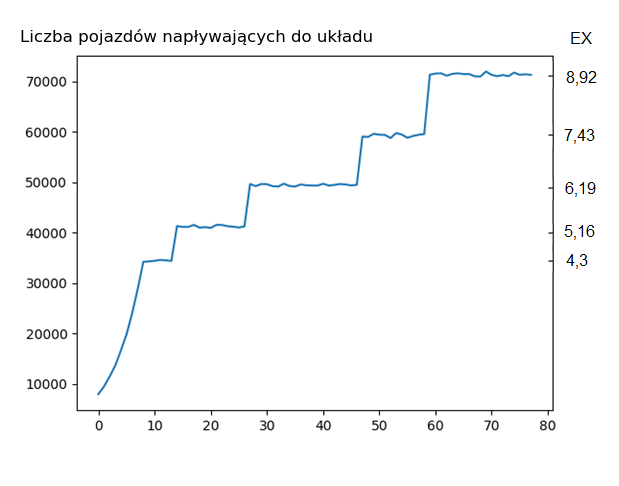
\includegraphics[width=14cm]{images/poli_wyniki/plot_cars_in}
	\label{fig:env_poli_in}
	\centering
	\caption{Wykres pojazdów napływających do układu}
\end{figure} \noindent
\begin{figure}[H]
	\centering
	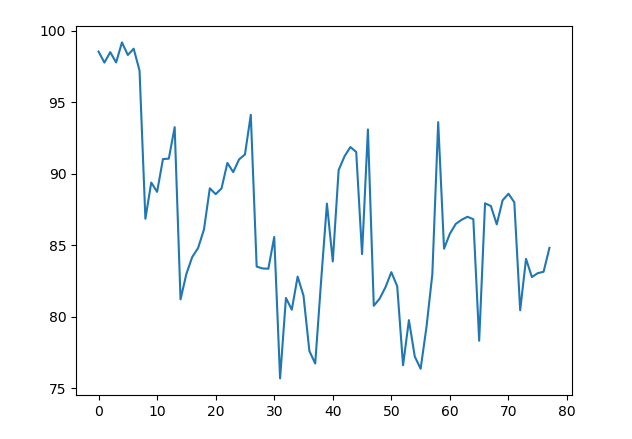
\includegraphics[width=13.5cm]{images/poli_wyniki/plot_cars_out_percentage_no_title}
	\label{fig:env_poli_out_percentage}
	\caption{Wykres procentowej części pojazdów opuszczających układ}
	\centering
\end{figure}
\begin{figure}[H]
	\centering
	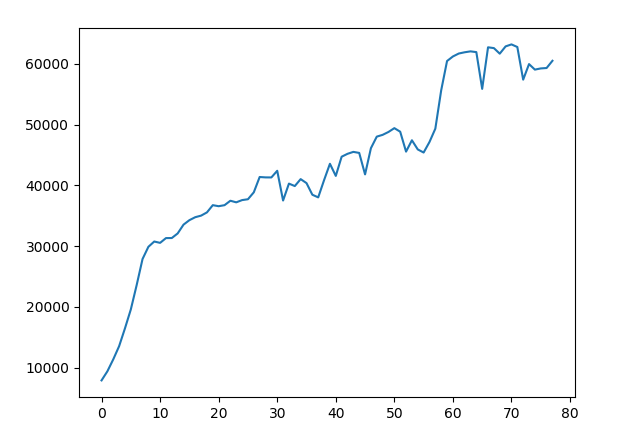
\includegraphics[width=13.5cm]{images/poli_wyniki/plot_cars_out_no_title}
	\label{fig:env_poli_out}
		\caption{Wykres liczby pojazdów opuszczających układ}
	\centering
\end{figure} \newpage
\noindent Poniższy wykres przedstawia zmianę wartości straty na zbiorze walidacyjnym sieci neuronowych poszczególnych agentów. Jest ona liczona jako błąd średniokwadratowy.
\begin{figure}[H]
	\centering
	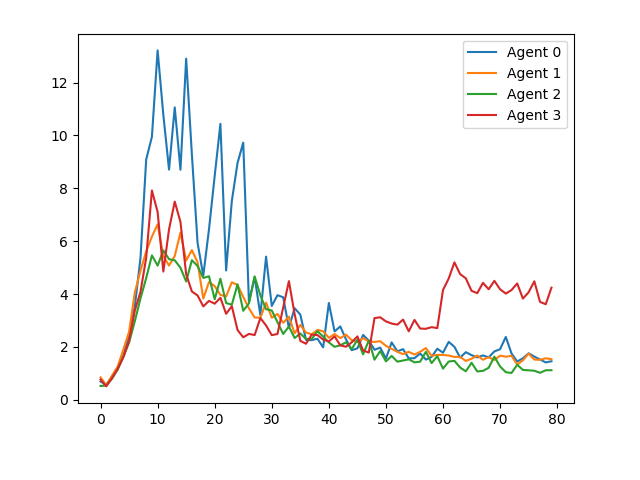
\includegraphics[width=14cm]{images/poli_wyniki/losses_no_title}
	\label{fig:losses}
	\caption{Wykres wartości funkcji straty na zbiorze walidacyjnym}
	\centering
\end{figure}

\chapter{Podsumowanie}

\indent \indent W pracy zostały przedstawione metody optymalizacji sygnalizacji świetlnej w środowisku drogowym o makroskopowym modelu ruchu. Są one oparte o metodę uczenia ze wzmocnieniem, przedstawioną jako Q-learning z wykorzystaniem sieci neuronowych. Początkową metodą optymalizacji był klasyczny Q-learning, który opiera się na tablicach. Metoda ta jednak nie została zastosowana z powodu słabego skalowania w środowiskach o większej przestrzeni stanu. 

Istotnym aspektem optymalizacji był dobór sygnału nagrody. Jako nagroda została wybrana liczba pojazdów, które właśnie opuściły skrzyżowanie. Zaletą tego rozwiązania jest wiedza na temat przyszłych nagród w przypadku fazy żółtych świateł (w trakcie których nie przejeżdża żaden pojazd). Zostało to wykorzystane do ustalenia wzoru \myref{eq:Q_DQN_II}. Często obieraną nagrodą jest ujemna liczba pojazdów czekających przed skrzyżowaniem \cite{rewards}. Nie mogłaby ona jednak zostać zastosowana wraz ze wzorem \myref{eq:Q_DQN_II}. Wydaje się  też być mniej wygodna pod względem diagnostyki wyników. Dodatkowym aspektem jest współdziałanie agentów w osiągnięciu założonego celu. W pracy \cite{wang2018cooperative} zostały przedstawione zasady systemu wieloagentowego. Pierwszą z nich jest realizacja założonego celu globalnego poprzez kooperacje agentów. Nagrody przyznawane agentom powinny służyć uzyskaniu celu globalnego. W tym przypadku jest to maksymalizacja liczby pojazdów opuszczających środowisko. Nagrody jednak nie muszą być modelowane bezpośrednio jako liczba pojazdów opuszczających układ. Natomiast powinny być one tak ukształtowane, aby osiągnąć cel globalny. 

Znaczącym problemem w trakcie doboru sposobu uczenia okazała się reprezentatywność danych. Początkowym ustawieniem było w pełni losowe zachowanie agentów w trakcie epizodów treningowych. Trwały one także równie długo, co testowe epizody. Konsekwencją tych ustaleń były stany z bardzo dużą liczbą pojazdów podczas epizodów treningowych. Agenci uczyli, jak zachowywać się w stanach,  gdy jest bardzo duża liczba pojazdów, bo takie były do nich głównie dostarczane dane. Rozwiązaniem tego problemu okazało się skrócenie długości epizodów treningowych i stosowanie od czasu do czasu akcji zachłannych. Epizody treningowe przypominały bardziej epizody testowe pod względem stanów, dzięki czemu sieć neuronowa miała do dyspozycji także bardziej odpowiednie dane.

Jako dalszy kierunek badań można upatrywać optymalizację doboru manewrów do faz.
Okazuje się, że jest to jednak dosyć wąskie zagadnienie.   Wykazane zostało w \cite{gottlich}, że najlepszy efekt przynosi wybranie najmniejszej możliwej liczby faz,  przy ograniczeniu, aby każdy manewr był obecny w przynajmniej jednej fazie. Ta metoda została wykorzystana w środowiskach rozdziału \ref{chapter:envs}.

Rozważane systemy ograniczały się do  ruchu pojazdów, jednak dalszy kierunek badań mógłby opierać się na uwzględnieniu także pieszych. Optymalizacja sygnalizacji świetlnej potencjalnie byłaby bardzo podobna do przedstawionej w niniejszej pracy. Stan dla każdego z agentów mógłby zawierać w sobie także informację na temat pieszych, czekających przed pasami. Dodatkowo nagroda powinna być modelowana z uwzględnieniem pieszych. 

Istotnym  tematem w kontekście eliminacji zatorów komunikacyjnych jest  obecnie  wykorzystanie sztucznej inteligencji  do kierowania ruchem  samochodami autonomicznymi .  Pojazdy te docelowo mają zapewnić przede wszystkim bardziej optymalną, bezwypadkową jazdę oraz dobór odpowiedniej trasy. Jest to jednak temat biegnący równolegle z optymalizacją sygnalizacji świetlnej.  Nadzieja na wyeliminowanie problemu zatorów może być pokładana w  dalszych badaniach nad sztuczną inteligencją ,  które będą uwzględniać obydwa wyżej wymienione kierunki.


\bibliographystyle{ieeetr}

\bibliography{refs}
\end{document}
